\chapter{جمع‌بندي و نتيجه‌گيري و پیشنهادات}

هدف این فصل سنجش عملکر کاهش بعد با استفاده از تصویر تصادفی است. بدین منظور برای هر یک از مجموعه داده‌های معرفی شده در فصل چهارم روش‌های مختلف کاهش بعد بوسیله تصویر تصادفی با پارامتر‌های مختلف مقایسه شده‌اند. هر سطر 
\autoref{tbl:1mx}
یک حالت مورد بررسی است که بر روی تمام مجموعه داده‌ی معرفی شده در فصل چهارم اعمال می‌شود. 

\begin{table}[H]
\centering\rowcolors{2}{gray!6}{white}
\caption{
شرایط کاهش بعد در شش بخش اول
}
\bigskip
\begin{tabular}{ccccc}
\hiderowcolors
\toprule
 & روش & پارامتر & مقدار پارامتر & بعد کاهش یافته\\
\midrule
\showrowcolors
\ref{sec:A2D2} &
پایدار & 
$\alpha$ &
 2(نرمال) & 2\\
\ref{sec:A2D3} &
پایدار & 
$\alpha$ &
 2(نرمال) & 3\\
\ref{sec:A1D2} &
پایدار & 
$\alpha$ &
 1(کوشی) & 2\\
\ref{sec:A1D3} &
پایدار & 
$\alpha$ &
 1(کوشی) & 3\\
\ref{sec:S2D2} &
گسسته & 
$s$ &
 2 & 2\\
\ref{sec:S2D3} &
گسسته & 
$s$ &
 2 & 3\\
\bottomrule
\end{tabular}
\rowcolors{2}{white}{white}
\label{tbl:1mx}
\end{table}




در شش بخش اول به بررسی عملکرد و پایداری کاهش بعد برای هر یک از سطرهای 
\autoref{tbl:1mx}
پرداختیم. عملکرد کاهش بعد با سنجه‌های 
$\mathrm{ARI}_d$
و 
$C_e$
که در (
\autoref{sec:ari_ce}
)
معرفی شده‌اند. در جدول ابتدای هر بخش برای مجموعه داده‌های مختلف سنجیده شده. در ادامه نمودار فراوانی 
$\mathrm{ARI}_d$
برای هر مجموعه داده بیان شده است که به طور شهودی انتظار ما را از عملکرد کاهش بعد با روش تصویر تصادفی بیان می‌کند. اگر نمودار فراوانی دارای قله‌های مشخصی باشد انتظار می‌رود که عملکرد کاهش بعد با روش تصویر تصادفی معنی‌دار باشد ولی اگر 
$\mathrm{ARI}_d$
دارای مقادیر انتظاری محتمل‌تری نباشد نمی‌توان انتظار داشت که با یک یا تعداد کمی کاهش بعد با ماتریس‌های تصادفی لزوما به عملکرد مشابهی مانند میانگین آماری بیان شده در جداول ابتدای هر بخش، دست یافت. مقادیر مربوط به جداول میانگین مربوط به 1000 ماتریس تصادفی مختلف است.

در چهار بخش بعدی رفتار عملکرد کاهش بعد (%
$C_e$%
) نسبت به پارامترهای مدل سنجیده شده است. برای حالت پایدار در دو حالت کاهش بعد به دو و سه بعد برای 
$\alpha$
از 1 تا 2 در قدم‌های 0.1 مقدار
$C_e$
با نمونه‌گیری 200 تایی بیان شده است. و برای کاهش بعد گسسته به دو و سه بعد برای 
$s$
از 1.5 تا 2.5 در قدم‌های 0.1 مقدار 
$C_e$
با نمونه‌گیری 200 تایی بیان شده است.



\section{
بررسی کاهش بعد نرمال
$(\alpha=2)$
به دو بعد
}
\label{sec:A2D2}

\subsection{جداول مقایسه عملکرد خوشه‌بندی}

\begin{table}[H]
\centering\rowcolors{2}{gray!6}{white}
\caption{
عملکرد تصویر تصادفی نرمال برای کاهش بعد به دو بعد
}
\bigskip
\begin{latin}
\begin{tabular}{lrrr}
\hiderowcolors
\toprule
Dataset & $ARI_p$ & $ARI_d$ & $C_e$\\
\midrule
\showrowcolors
Thyroid & 0.5831656 & 0.3989981 & -18\\
Iris & 0.6201352 & 0.4710315 & -15\\
Diabetes & 0.3801662 & 0.3647537 & -2\\
Swiss Banknotes & 0.8456292 & 0.3880871 & -46\\
Seeds & 0.7732937 & 0.4482112 & -33\\
\addlinespace
Crabs & 0.0481402 & 0.0439549 & 0\\
Mice Protein Expression & 0.1316117 & 0.0657659 & -7\\
\bottomrule
\end{tabular}
\end{latin}
\rowcolors{2}{white}{white}
\end{table}


\subsection{نمودار فراوانی عملکرد خوشه‌بندی}


\begin{figure}[H]
\centering
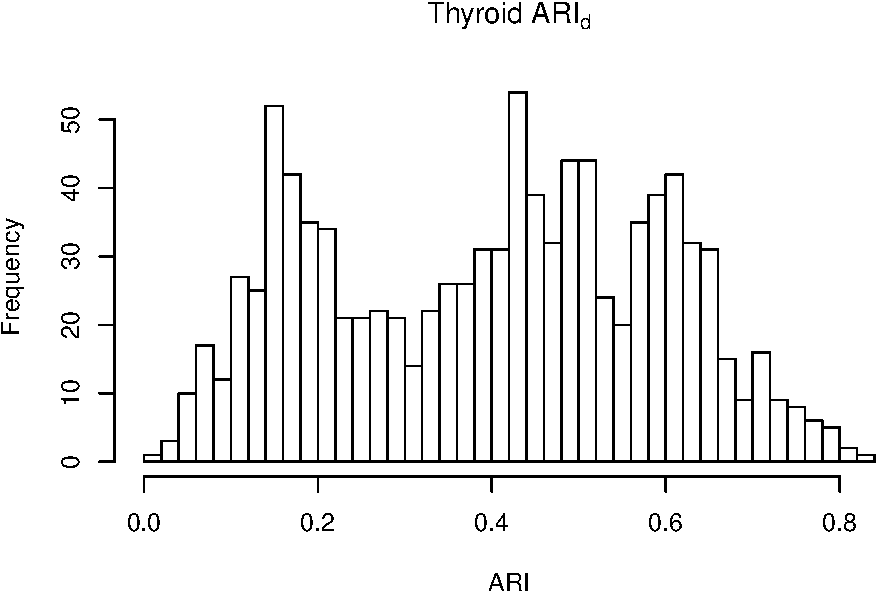
\includegraphics[width=0.7\linewidth]{Report_files/figure-latex/unnamed-chunk-3-1} 
\caption{
نمودار فراوانی عملکرد خوشه‌بندی 
$\mathrm{ARI}_d$
پس از کاهش بعد با استفاده از تصویر تصادفی
نرمال (%
$\alpha=2$%
)
به دو (%
$d=2$%
)
بعد برای مجموعه داده‌های
تیروئید
\ref{sec:Thyroid}
. این نمودار فراوانی،
قله‌های
مشخصی را نشان 
می‌دهد
و مقادیر آن طیف 
وسیعی را پوشش می‌دهند.
}
\end{figure}

\begin{figure}[H]
\centering
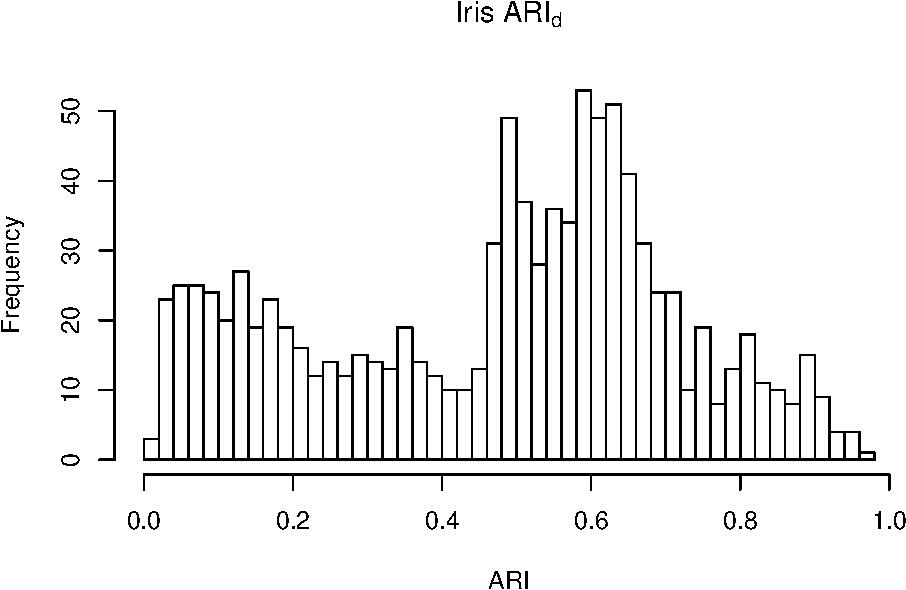
\includegraphics[width=0.7\linewidth]{Report_files/figure-latex/unnamed-chunk-3-2}
\caption{
نمودار فراوانی عملکرد خوشه‌بندی 
$\mathrm{ARI}_d$
پس از کاهش بعد با استفاده از تصویر تصادفی
نرمال (%
$\alpha=2$%
)
به دو (%
$d=2$%
)
بعد برای مجموعه داده‌های
آیریس
\ref{sec:Iris}
این نمودار فراوانی،
قله
مشخصی را نشان 
می‌دهد
و دسته‌ای از مقادیر آن طیف 
محدودی
را پوشش می‌دهند که امکان این را فراهم می‌آورد که با تست تعداد محدودی ماتریس تصادفی کاهش بعد قابل قبولی را انتظار داشته باشیم.
}
\end{figure}

\begin{figure}[H]
\centering
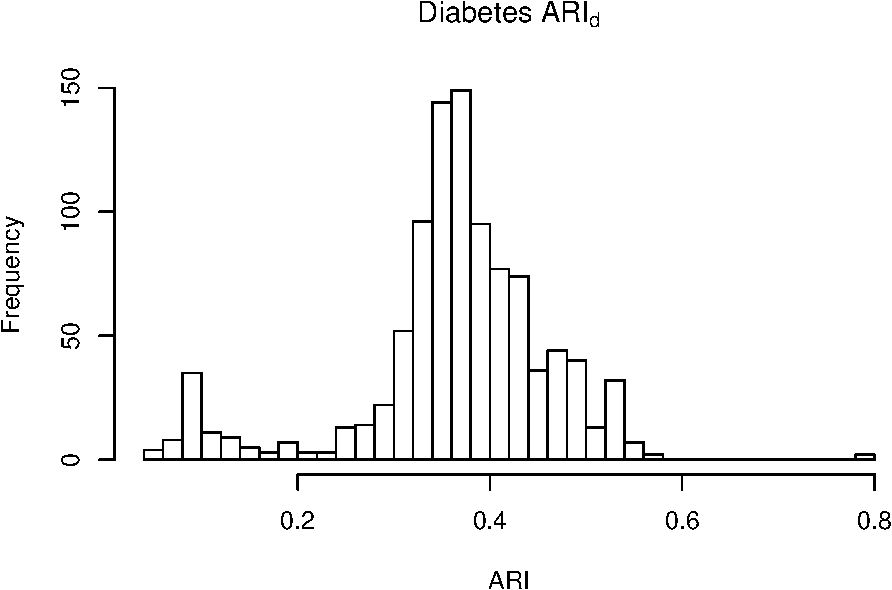
\includegraphics[width=0.7\linewidth]{Report_files/figure-latex/unnamed-chunk-3-3}
\caption{
نمودار فراوانی عملکرد خوشه‌بندی 
$\mathrm{ARI}_d$
پس از کاهش بعد با استفاده از تصویر تصادفی
نرمال (%
$\alpha=2$%
)
به دو (%
$d=2$%
)
بعد برای مجموعه داده‌های
دیابت
\ref{sec:Diabetes}
این نمودار فراوانی،
قله
مشخصی را نشان 
می‌دهد
و مقادیر آن طیف 
محدودی
را پوشش می‌دهند.
}
\end{figure}



\begin{figure}[H]
\centering
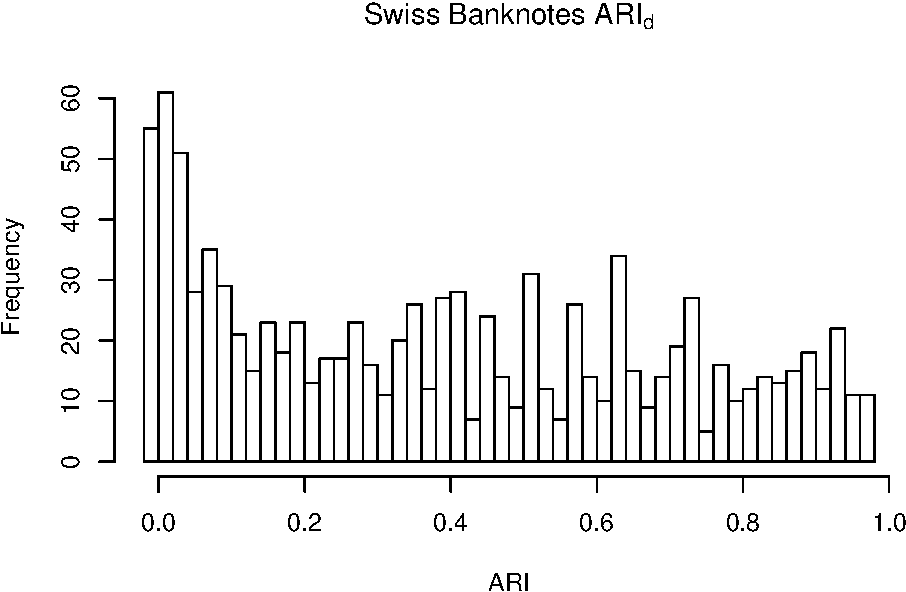
\includegraphics[width=0.7\linewidth]{Report_files/figure-latex/unnamed-chunk-3-4}
\caption{
نمودار فراوانی عملکرد خوشه‌بندی 
$\mathrm{ARI}_d$
پس از کاهش بعد با استفاده از تصویر تصادفی
نرمال (%
$\alpha=2$%
)
به دو (%
$d=2$%
)
بعد برای مجموعه داده‌های
اسکناس
\ref{sec:Swiss}
این نمودار فراوانی،
قله
مشخصی را نشان 
نمی‌دهد
و مقادیر آن طیف 
وسیعی را پوشش می‌دهند.
}
\end{figure}

\begin{figure}[H]
\centering
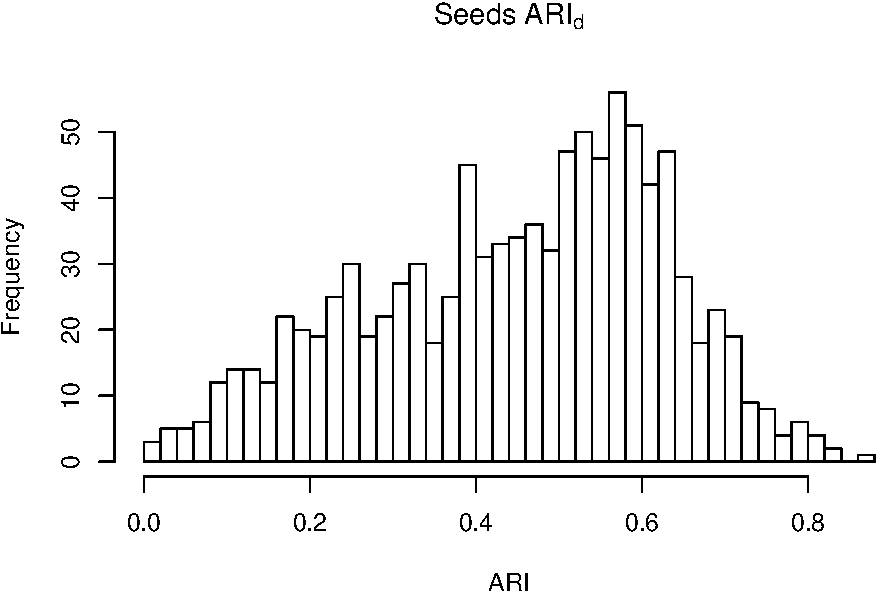
\includegraphics[width=0.7\linewidth]{Report_files/figure-latex/unnamed-chunk-3-5}
\caption{
نمودار فراوانی عملکرد خوشه‌بندی 
$\mathrm{ARI}_d$
پس از کاهش بعد با استفاده از تصویر تصادفی
نرمال (%
$\alpha=2$%
)
به دو (%
$d=2$%
)
بعد برای مجموعه داده‌های
بذر
\ref{sec:Seeds}
این نمودار فراوانی،
قله
مشخصی را نشان 
می‌دهد
و مقادیر آن طیف 
محدودی
را پوشش می‌دهند.
}
\end{figure}

\begin{figure}[H]
\centering
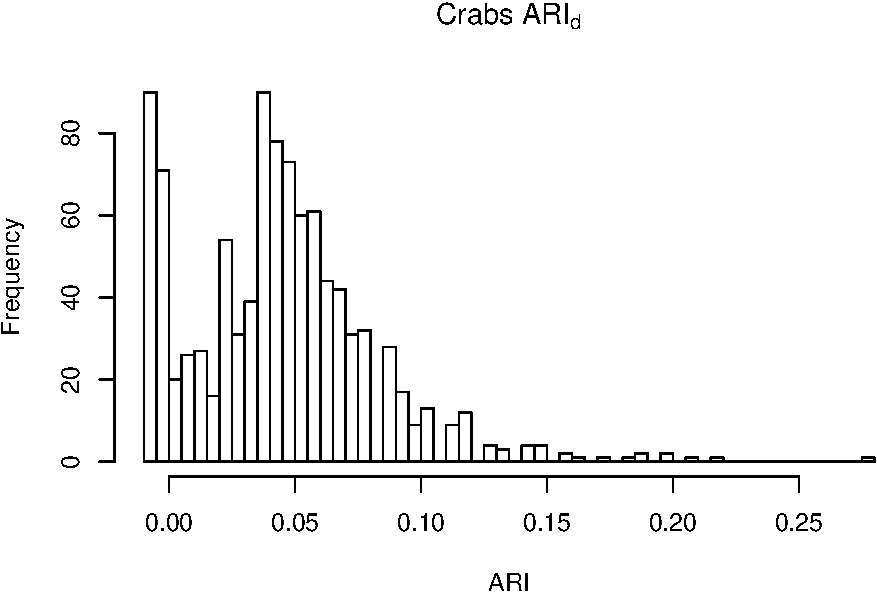
\includegraphics[width=0.7\linewidth]{Report_files/figure-latex/unnamed-chunk-3-6}
\caption{
نمودار فراوانی عملکرد خوشه‌بندی 
$\mathrm{ARI}_d$
پس از کاهش بعد با استفاده از تصویر تصادفی
نرمال (%
$\alpha=2$%
)
به دو (%
$d=2$%
)
بعد برای مجموعه داده‌های
خرچنگ
\ref{sec:Crabs}
این نمودار فراوانی،
قله
مشخصی را نشان 
می‌دهد
و مقادیر آن طیف 
محدودی
را پوشش می‌دهند.
}
\end{figure}

\begin{figure}[H]
\centering
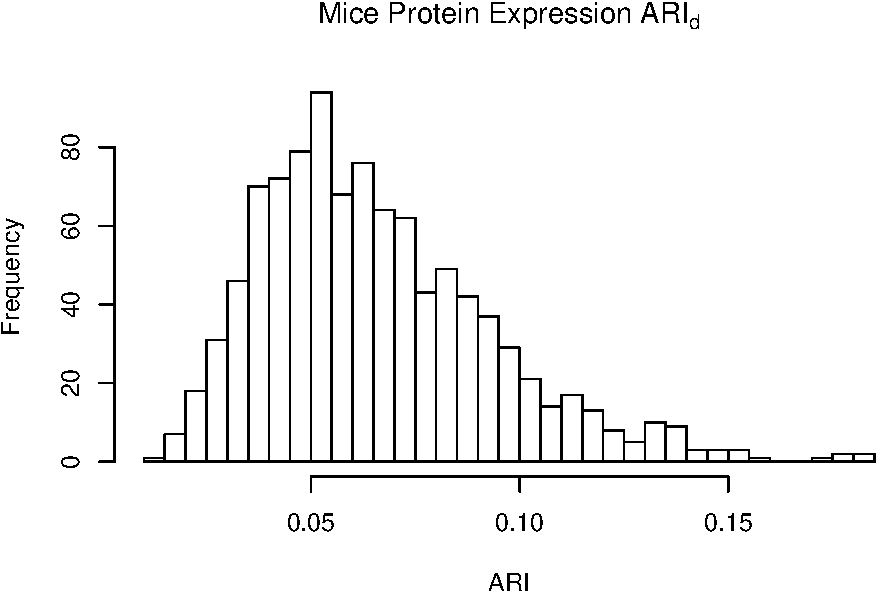
\includegraphics[width=0.7\linewidth]{Report_files/figure-latex/unnamed-chunk-3-7}
\caption{
نمودار فراوانی عملکرد خوشه‌بندی 
$\mathrm{ARI}_d$
پس از کاهش بعد با استفاده از تصویر تصادفی
نرمال (%
$\alpha=2$%
)
به دو (%
$d=2$%
)
بعد برای مجموعه داده‌های
پروتئین
\ref{sec:MPE}
این نمودار فراوانی،
قله
مشخصی را نشان 
می‌دهد
و مقادیر آن طیف 
محدودی
را پوشش می‌دهند.
}
\end{figure}








\section{نتایج برای کاهش بعد نرمال به سه بعد}
\label{sec:A2D3}

\subsection{جداول مقایسه عملکرد خوشه‌بندی}


\begin{table}[H]
\caption{
عملکرد تصویر تصادفی نرمال برای کاهش بعد به سه بعد
}
\bigskip
\centering\rowcolors{2}{gray!6}{white}
\begin{latin}
\begin{tabular}{lrrr}
\hiderowcolors
\toprule
Dataset & $ARI_p$ & $ARI_d$ & $C_e$\\
\midrule
\showrowcolors
Thyroid & 0.5831656 & 0.4344288 & -15\\
Iris & 0.6201352 & 0.5359746 & -8\\
Swiss Banknotes & 0.8456292 & 0.4714675 & -37\\
Seeds & 0.7732937 & 0.5299329 & -24\\
\addlinespace
Mice Protein Expression & 0.1316575 & 0.0814613 & -5\\
Crabs & 0.0481402 & 0.0485252 & 0\\
\bottomrule
\end{tabular}
\end{latin}
\rowcolors{2}{white}{white}
\end{table}


\subsection{نمودار فراوانی عملکرد خوشه‌بندی}


\begin{figure}[H]
\centering
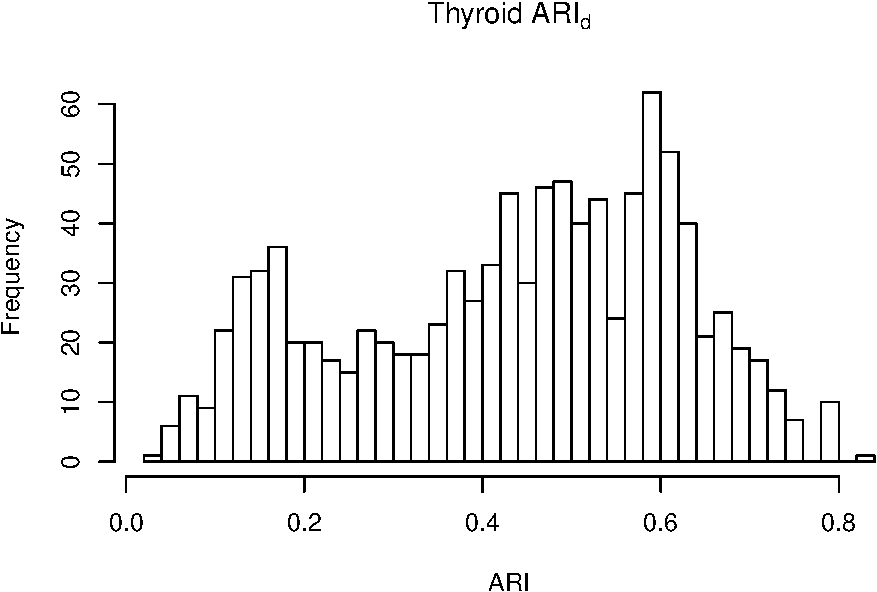
\includegraphics[width=0.7\linewidth]{Report_files/figure-latex/unnamed-chunk-6-1}
\caption{
نمودار فراوانی عملکرد خوشه‌بندی 
$\mathrm{ARI}_d$
پس از کاهش بعد با استفاده از تصویر تصادفی
نرمال (%
$\alpha=2$%
)
به 
سه (%
$d=3$%
)
بعد برای مجموعه داده‌های
تیروئید
\ref{sec:Thyroid}
این نمودار فراوانی،
قله
مشخصی را نشان 
می‌دهد
و مقادیر آن طیف 
محدودی
را پوشش می‌دهند.
}
\end{figure}


\begin{figure}[H]
\centering
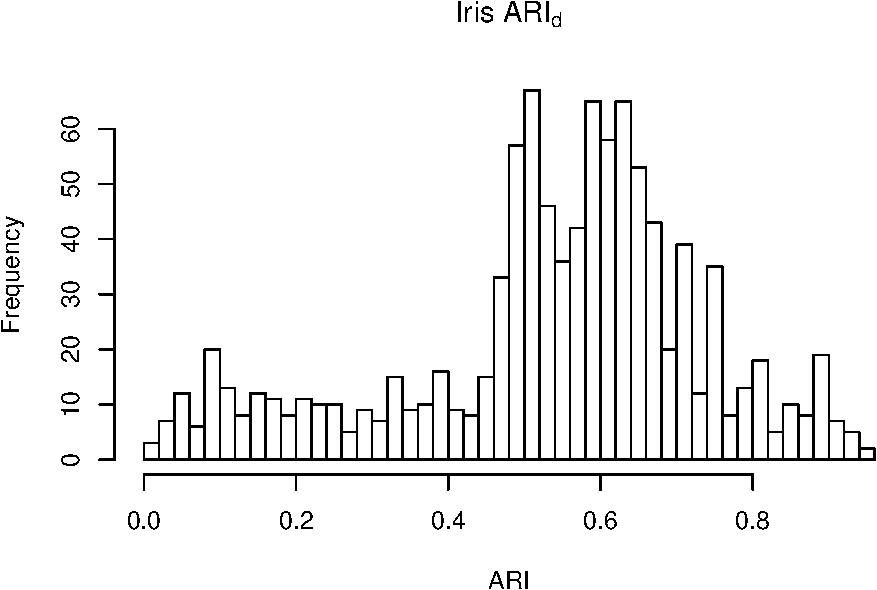
\includegraphics[width=0.7\linewidth]{Report_files/figure-latex/unnamed-chunk-6-2}
\caption{
نمودار فراوانی عملکرد خوشه‌بندی 
$\mathrm{ARI}_d$
پس از کاهش بعد با استفاده از تصویر تصادفی
نرمال (%
$\alpha=2$%
)
به
سه (%
$d=3$%
)
بعد برای مجموعه داده‌های
آیریس
\ref{sec:Iris}
این نمودار فراوانی،
قله
مشخصی را نشان 
می‌دهد
و مقادیر آن طیف 
محدودی
را پوشش می‌دهند.
}
\end{figure}


\begin{figure}[H]
\centering
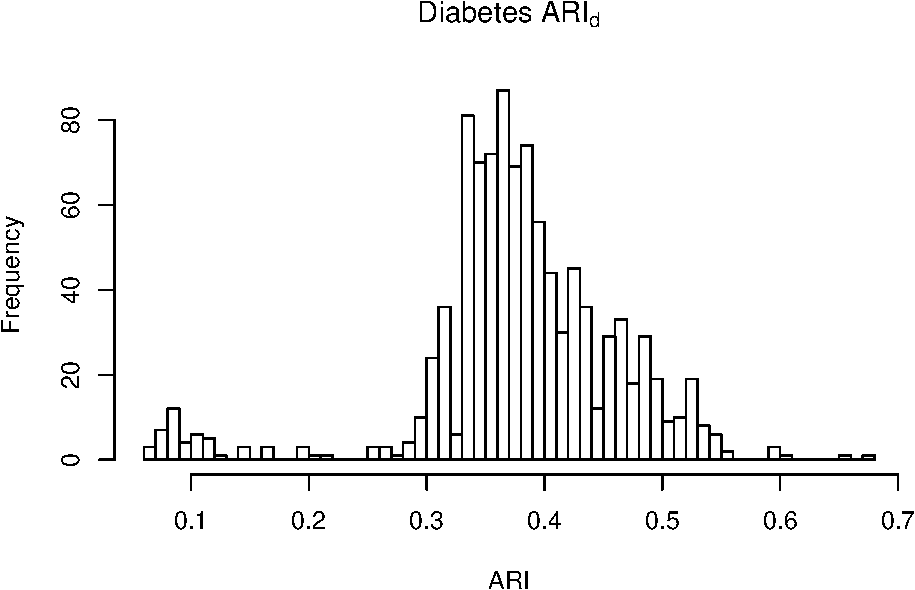
\includegraphics[width=0.7\linewidth]{Report_files/figure-latex/unnamed-chunk-6-3}
\caption{
نمودار فراوانی عملکرد خوشه‌بندی 
$\mathrm{ARI}_d$
پس از کاهش بعد با استفاده از تصویر تصادفی
نرمال (%
$\alpha=2$%
)
سه (%
$d=3$%
)
بعد برای مجموعه داده‌های
دیابت
\ref{sec:Diabetes}
این نمودار فراوانی،
قله
مشخصی را نشان 
می‌دهد
و مقادیر آن طیف 
محدودی
 را پوشش می‌دهند.
}
\end{figure}


\begin{figure}[H]
\centering
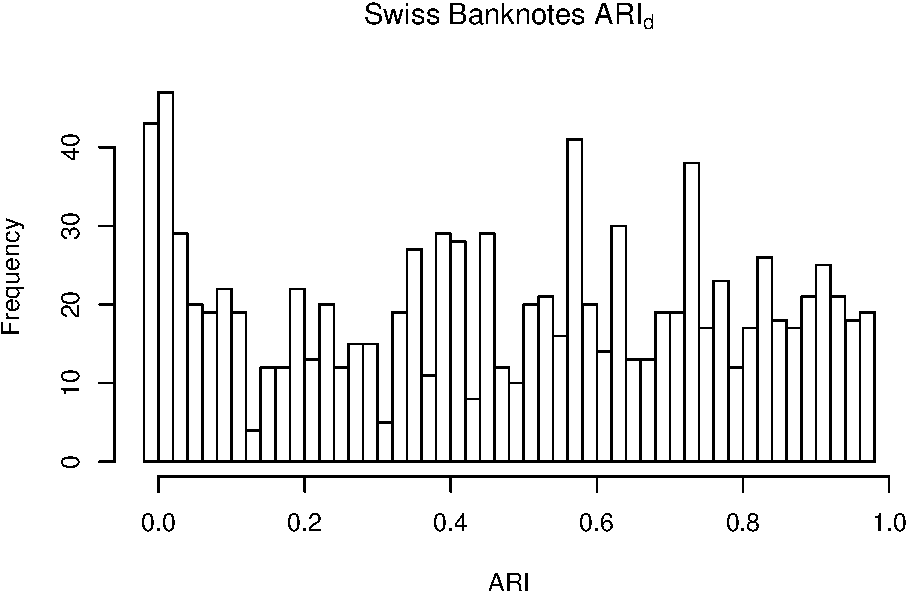
\includegraphics[width=0.7\linewidth]{Report_files/figure-latex/unnamed-chunk-6-4}
\caption{
نمودار فراوانی عملکرد خوشه‌بندی 
$\mathrm{ARI}_d$
پس از کاهش بعد با استفاده از تصویر تصادفی
نرمال (%
$\alpha=2$%
)
به
سه (%
$d=3$%
)
بعد برای مجموعه داده‌های
اسکناس
\ref{sec:Swiss}
این نمودار فراوانی،
قله
مشخصی را نشان 
نمی‌دهد
و مقادیر آن طیف 
وسیعی را پوشش می‌دهند.
}
\end{figure}


\begin{figure}[H]
\centering
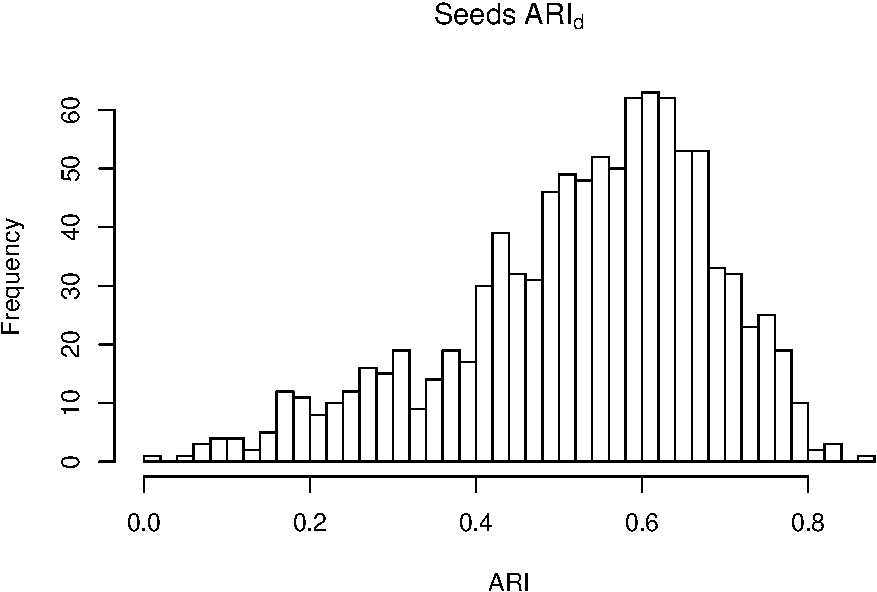
\includegraphics[width=0.7\linewidth]{Report_files/figure-latex/unnamed-chunk-6-5}
\caption{
نمودار فراوانی عملکرد خوشه‌بندی 
$\mathrm{ARI}_d$
پس از کاهش بعد با استفاده از تصویر تصادفی
نرمال (%
$\alpha=2$%
)
به سه (%
$d=3$%
)
بعد برای مجموعه داده‌های
بذر
\ref{sec:Seeds}
این نمودار فراوانی،
قله
مشخصی را نشان 
می‌دهد
و مقادیر آن طیف 
محدودی
را پوشش می‌دهند.
}
\end{figure}


\begin{figure}[H]
\centering
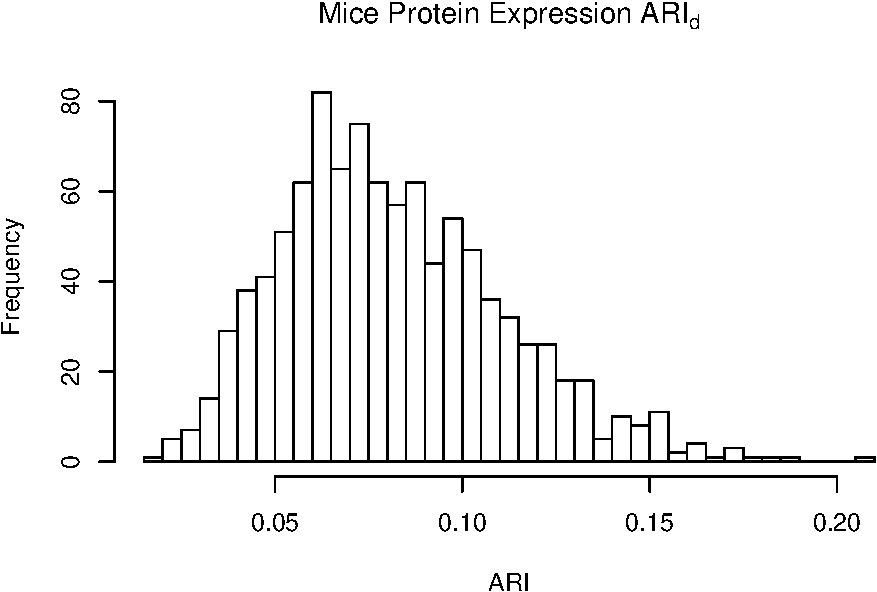
\includegraphics[width=0.7\linewidth]{Report_files/figure-latex/unnamed-chunk-6-6}
\caption{
نمودار فراوانی عملکرد خوشه‌بندی 
$\mathrm{ARI}_d$
پس از کاهش بعد با استفاده از تصویر تصادفی
نرمال (%
$\alpha=2$%
)
به سه (%
$d=3$%
)
بعد برای مجموعه داده‌های
پروتئین
\ref{sec:MPE}
این نمودار فراوانی،
قله
مشخصی را نشان 
می‌دهد
و مقادیر آن طیف 
محدودی
 را پوشش می‌دهند.
}
\end{figure}

\begin{figure}[H]
\centering
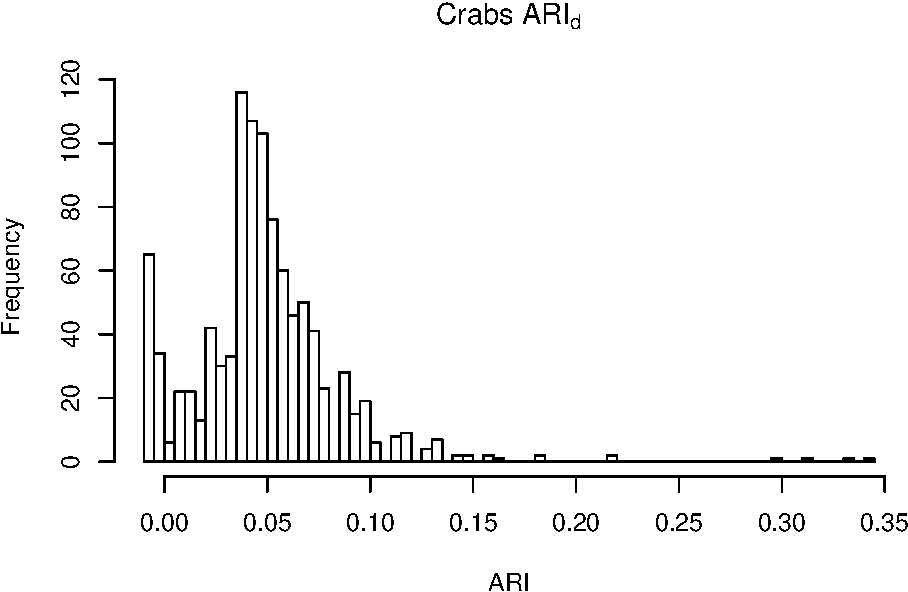
\includegraphics[width=0.7\linewidth]{Report_files/figure-latex/unnamed-chunk-6-7}
\caption{
نمودار فراوانی عملکرد خوشه‌بندی 
$\mathrm{ARI}_d$
پس از کاهش بعد با استفاده از تصویر تصادفی
نرمال (%
$\alpha=2$%
)
به سه (%
$d=3$%
)
بعد برای مجموعه داده‌های
خرچنگ
\ref{sec:Crabs}
این نمودار فراوانی،
قله
مشخصی را نشان 
می‌دهد
و مقادیر آن طیف 
محدودی
 را پوشش می‌دهند.
}
\end{figure}








\section{
نتایج برای کاهش بعد کوشی 
$(\alpha = 1)$
به دو بعد
}
\label{sec:A1D2}

\subsection{جداول مقایسه عملکرد خوشه‌بندی}


\begin{table}[H]
\caption{
عملکرد تصویر تصادفی کوشی برای کاهش بعد به دو بعد
}
\bigskip
\centering\rowcolors{2}{gray!6}{white}
\begin{latin}
\begin{tabular}{lrrr}
\hiderowcolors
\toprule
Dataset & $ARI_p$ & $ARI_d$ & $C_e$\\
\midrule
\showrowcolors
Thyroid & 0.5831656 & 0.3559301 & -23\\
Iris & 0.6201352 & 0.5078172 & -11\\
Diabetes & 0.3801662 & 0.3341399 & -5\\
Swiss Banknotes & 0.8456292 & 0.4011119 & -44\\
Seeds & 0.7732937 & 0.4488349 & -32\\
\addlinespace
Mice Protein Expression & 0.1317342 & 0.0592468 & -7\\
Crabs & 0.0481402 & 0.0469365 & 0\\
\bottomrule
\end{tabular}
\end{latin}
\rowcolors{2}{white}{white}
\end{table}


\subsection{نمودار فراوانی عملکرد خوشه‌بندی}


\begin{figure}[H]
\centering
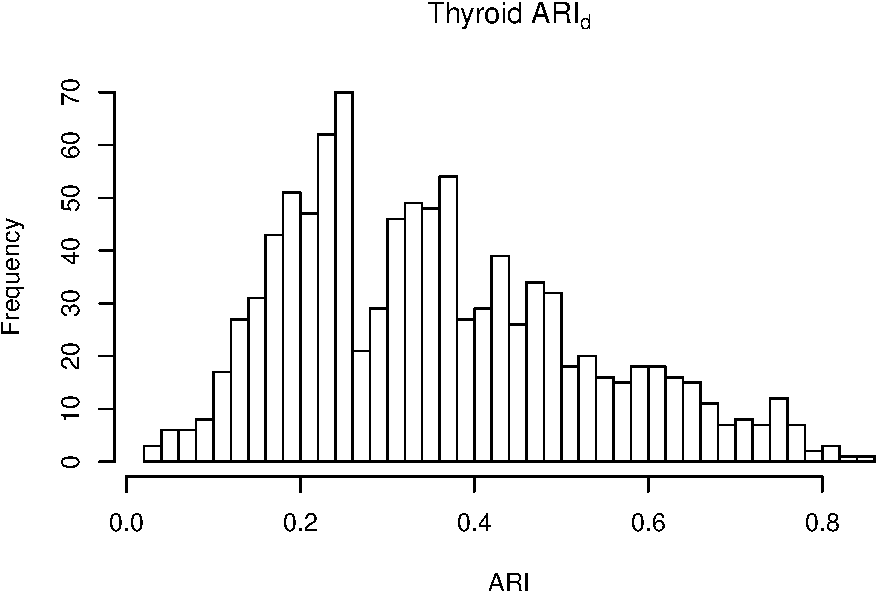
\includegraphics[width=0.7\linewidth]{Report_files/figure-latex/unnamed-chunk-9-1}
\caption{
نمودار فراوانی عملکرد خوشه‌بندی 
$\mathrm{ARI}_d$
پس از کاهش بعد با استفاده از تصویر تصادفی
کوشی (%
$\alpha=1$%
)
به دو (%
$d=2$%
)
بعد برای مجموعه داده‌های
تیروئید
\ref{sec:Thyroid}
این نمودار فراوانی،
قله
مشخصی را نشان 
می‌دهد
و مقادیر آن طیف 
محدودی
 را پوشش می‌دهند.
}
\end{figure}


\begin{figure}[H]
\centering
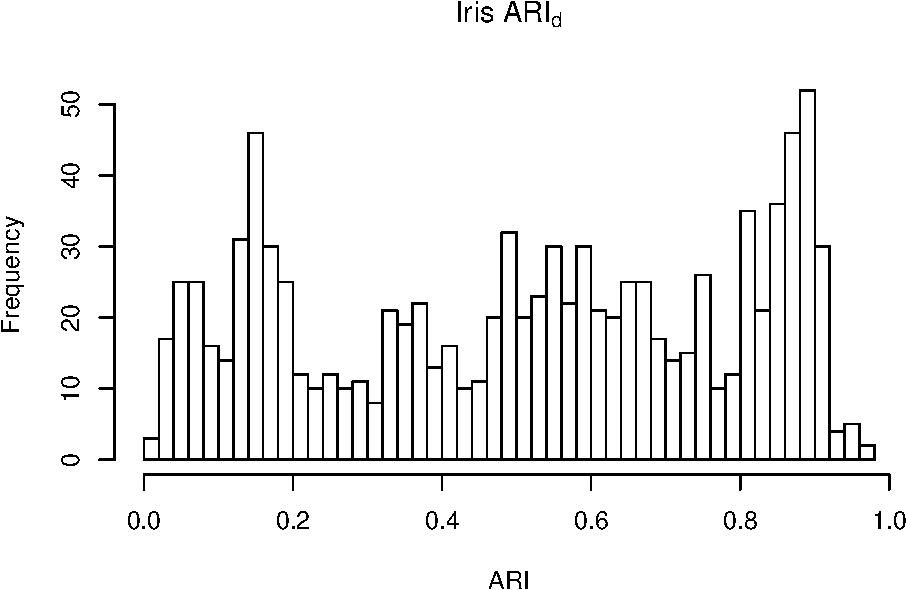
\includegraphics[width=0.7\linewidth]{Report_files/figure-latex/unnamed-chunk-9-2}
\caption{
نمودار فراوانی عملکرد خوشه‌بندی 
$\mathrm{ARI}_d$
پس از کاهش بعد با استفاده از تصویر تصادفی
کوشی (%
$\alpha=1$%
)
به دو (%
$d=2$%
)
بعد برای مجموعه داده‌های
آیریس
\ref{sec:Iris}
این نمودار فراوانی،
قله
مشخصی را نشان 
می‌دهد
و مقادیر آن طیف 
وسیعی را پوشش می‌دهند.
}
\end{figure}


\begin{figure}[H]
\centering
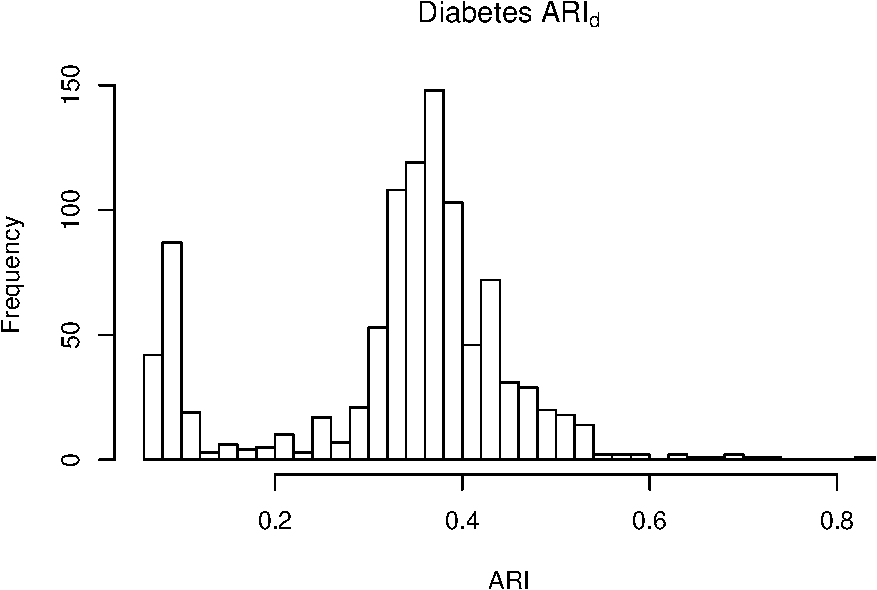
\includegraphics[width=0.7\linewidth]{Report_files/figure-latex/unnamed-chunk-9-3}
\caption{
نمودار فراوانی عملکرد خوشه‌بندی 
$\mathrm{ARI}_d$
پس از کاهش بعد با استفاده از تصویر تصادفی
کوشی (%
$\alpha=1$%
)
به دو (%
$d=2$%
)
بعد برای مجموعه داده‌های
دیابت
\ref{sec:Diabetes}
این نمودار فراوانی،
قله‌های
مشخصی را نشان 
می‌دهد
و مقادیر آن طیف 
محدودی
 را پوشش می‌دهند.
}
\end{figure}


\begin{figure}[H]
\centering
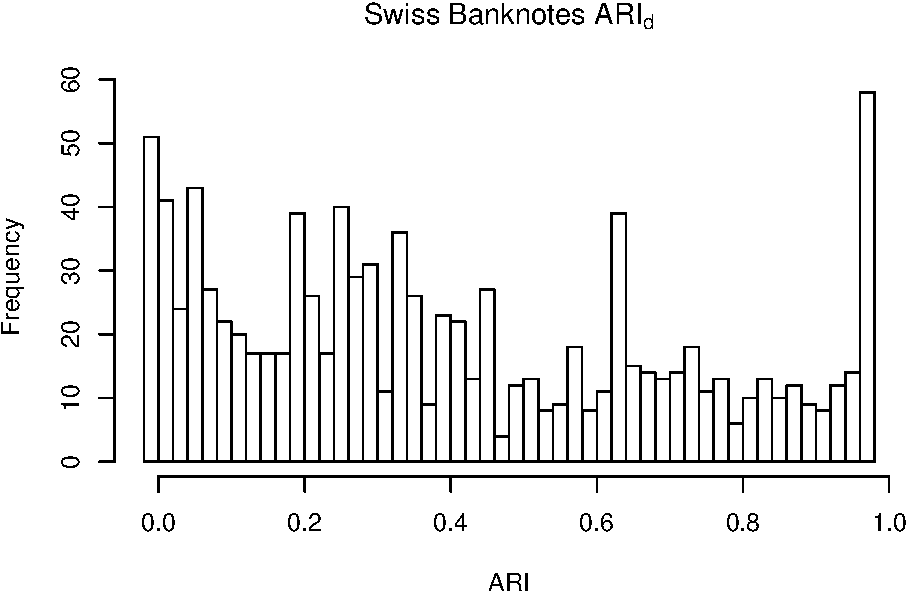
\includegraphics[width=0.7\linewidth]{Report_files/figure-latex/unnamed-chunk-9-4}
\caption{
نمودار فراوانی عملکرد خوشه‌بندی 
$\mathrm{ARI}_d$
پس از کاهش بعد با استفاده از تصویر تصادفی
کوشی (%
$\alpha=1$%
)
به دو (%
$d=2$%
)
بعد برای مجموعه داده‌های
اسکناس
\ref{sec:Swiss}
این نمودار فراوانی،
قله
مشخصی را نشان 
نمی‌دهد
و مقادیر آن طیف 
وسیعی را پوشش می‌دهند.
}
\end{figure}


\begin{figure}[H]
\centering
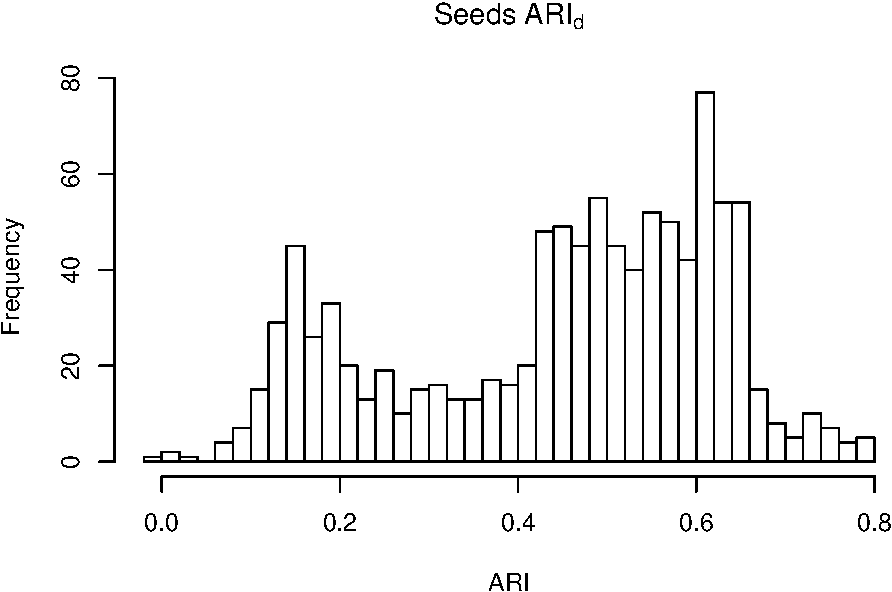
\includegraphics[width=0.7\linewidth]{Report_files/figure-latex/unnamed-chunk-9-5}
\caption{
نمودار فراوانی عملکرد خوشه‌بندی 
$\mathrm{ARI}_d$
پس از کاهش بعد با استفاده از تصویر تصادفی
کوشی (%
$\alpha=1$%
)
به دو (%
$d=2$%
)
بعد برای مجموعه داده‌های
بذر
\ref{sec:Seeds}
این نمودار فراوانی،
قله‌های
مشخصی را نشان 
می‌دهد
و مقادیر آن طیف 
وسیعی را پوشش می‌دهند.
}
\end{figure}


\begin{figure}[H]
\centering
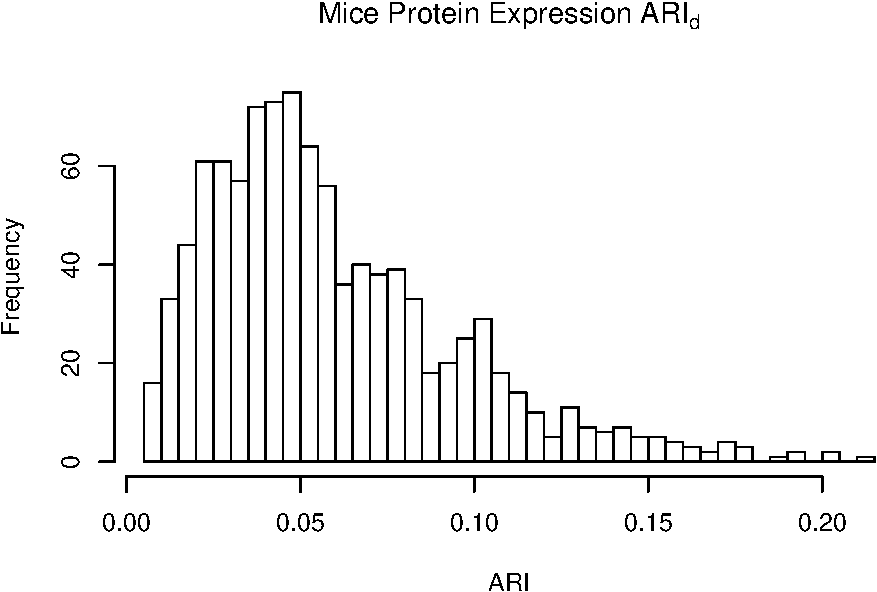
\includegraphics[width=0.7\linewidth]{Report_files/figure-latex/unnamed-chunk-9-6}
\caption{
نمودار فراوانی عملکرد خوشه‌بندی 
$\mathrm{ARI}_d$
پس از کاهش بعد با استفاده از تصویر تصادفی
کوشی (%
$\alpha=1$%
)
به دو (%
$d=2$%
)
بعد برای مجموعه داده‌های
پروتئین
\ref{sec:MPE}
این نمودار فراوانی،
قله
مشخصی را نشان 
می‌دهد
و مقادیر آن طیف 
محدودی
 را پوشش می‌دهند.
}
\end{figure}


\begin{figure}[H]
\centering
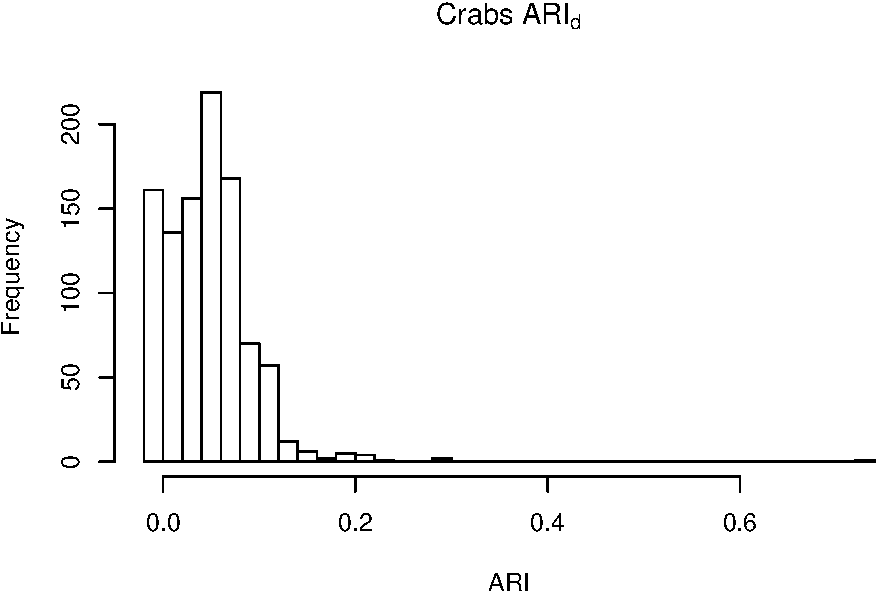
\includegraphics[width=0.7\linewidth]{Report_files/figure-latex/unnamed-chunk-9-7}
\caption{
نمودار فراوانی عملکرد خوشه‌بندی 
$\mathrm{ARI}_d$
پس از کاهش بعد با استفاده از تصویر تصادفی
کوشی (%
$\alpha=1$%
)
به دو (%
$d=2$%
)
بعد برای مجموعه داده‌های
خرچنگ
\ref{sec:Crabs}
این نمودار فراوانی،
قله
مشخصی را نشان 
می‌دهد
و مقادیر آن طیف 
محدودی
 را پوشش می‌دهند.
}
\end{figure}







\section{نتایج برای کاهش بعد کوشی به سه بعد}
\label{sec:A1D3}

\subsection{جداول مقایسه عملکرد خوشه‌بندی}

\begin{table}[H]
\caption{
عملکرد تصویر تصادفی کوشی برای کاهش بعد به سه بعد
}
\bigskip
\centering\rowcolors{2}{gray!6}{white}
\begin{latin}
\begin{tabular}{lrrr}
\hiderowcolors
\toprule
Dataset & $ARI_p$ & $ARI_d$ & $C_e$\\
\midrule
\showrowcolors
Thyroid & 0.5831656 & 0.3658900 & -22\\
Iris & 0.6201352 & 0.5441285 & -8\\
Swiss Banknotes & 0.8456292 & 0.4330544 & -41\\
Seeds & 0.7732937 & 0.4697687 & -30\\
\addlinespace
Mice Protein Expression & 0.1317362 & 0.0659775 & -7\\
Crabs & 0.0481402 & 0.0452313 & 0\\
\bottomrule
\end{tabular}
\end{latin}
\rowcolors{2}{white}{white}
\end{table}


\subsection{نمودار فراوانی عملکرد خوشه‌بندی}

\begin{figure}[H]
\centering
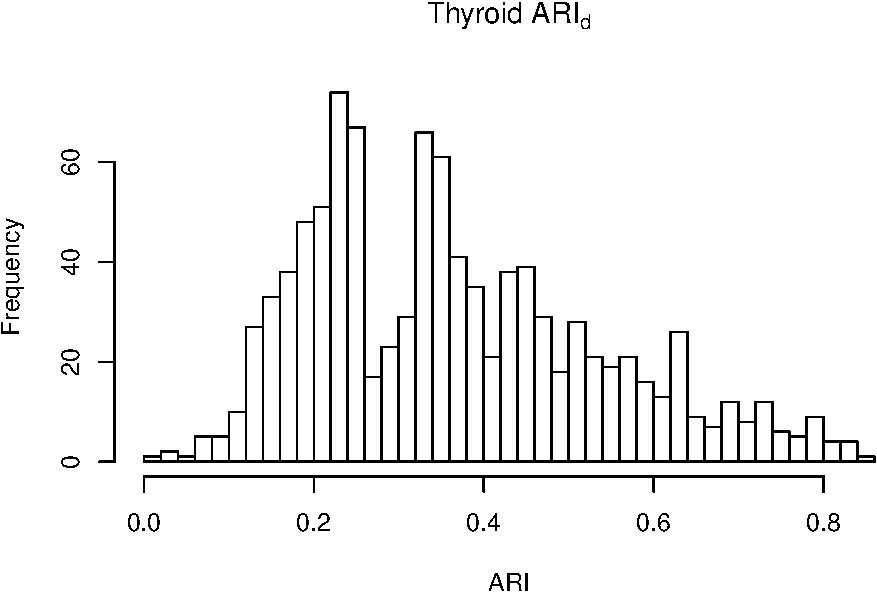
\includegraphics[width=0.7\linewidth]{Report_files/figure-latex/unnamed-chunk-12-1}
\caption{
نمودار فراوانی عملکرد خوشه‌بندی 
$\mathrm{ARI}_d$
پس از کاهش بعد با استفاده از تصویر تصادفی
کوشی (%
$\alpha=1$%
)
به
سه (%
$d=3$%
)
بعد برای مجموعه داده‌های
دیابت
\ref{sec:Diabetes}
این نمودار فراوانی،
قله‌های
مشخصی را نشان 
می‌دهد
و مقادیر آن طیف 
وسیعی را پوشش می‌دهند.
}
\end{figure}

\begin{figure}[H]
\centering
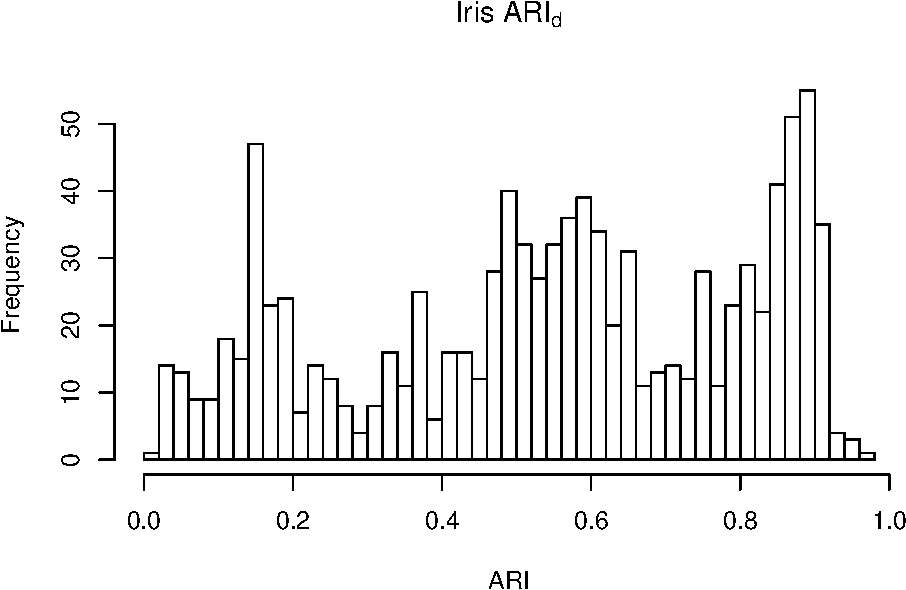
\includegraphics[width=0.7\linewidth]{Report_files/figure-latex/unnamed-chunk-12-2}
\caption{
نمودار فراوانی عملکرد خوشه‌بندی 
$\mathrm{ARI}_d$
پس از کاهش بعد با استفاده از تصویر تصادفی
کوشی (%
$\alpha=1$%
)
به
سه (%
$d=3$%
)
بعد برای مجموعه داده‌های
آیریس
\ref{sec:Iris}
این نمودار فراوانی،
قله
مشخصی را نشان 
نمی‌دهد
و مقادیر آن طیف 
وسیعی را پوشش می‌دهند.
}
\end{figure}

\begin{figure}[H]
\centering
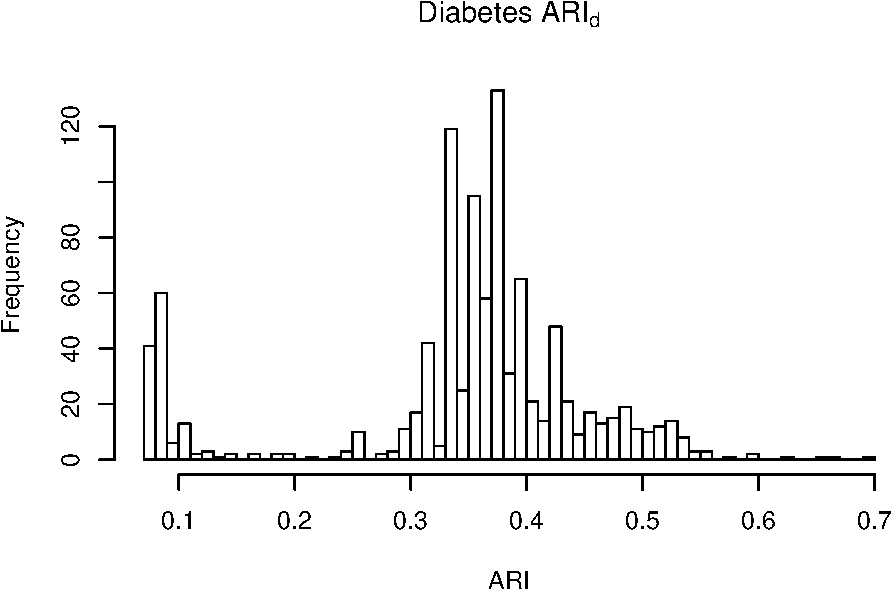
\includegraphics[width=0.7\linewidth]{Report_files/figure-latex/unnamed-chunk-12-3}
\caption{
نمودار فراوانی عملکرد خوشه‌بندی 
$\mathrm{ARI}_d$
پس از کاهش بعد با استفاده از تصویر تصادفی
کوشی (%
$\alpha=1$%
)
به 
سه (%
$d=3$%
)
بعد برای مجموعه داده‌های
دیابت
\ref{sec:Diabetes}
این نمودار فراوانی،
قله
مشخصی را نشان 
می‌دهد
و مقادیر آن طیف 
محدودی
 را پوشش می‌دهند.
}
\end{figure}

\begin{figure}[H]
\centering
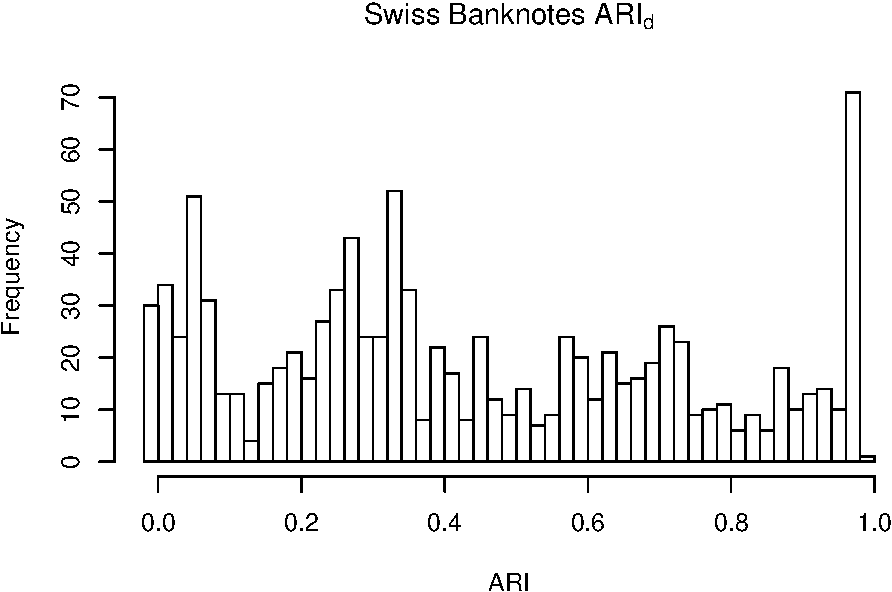
\includegraphics[width=0.7\linewidth]{Report_files/figure-latex/unnamed-chunk-12-4}
\caption{
نمودار فراوانی عملکرد خوشه‌بندی 
$\mathrm{ARI}_d$
پس از کاهش بعد با استفاده از تصویر تصادفی
کوشی (%
$\alpha=1$%
)
به 
سه (%
$d=3$%
)
بعد برای مجموعه داده‌های
اسکناس
\ref{sec:Swiss}
این نمودار فراوانی،
قله‌های
مشخصی را نشان 
می‌دهد
و مقادیر آن طیف 
وسیعی را پوشش می‌دهند. در این نمودار موضوع جالب برخی از تصویر‌های تصادفی هستند که عملکردی نزدیک به عملکرد حالت کاهش نیافته دارند.
}
\end{figure}

\begin{figure}[H]
\centering
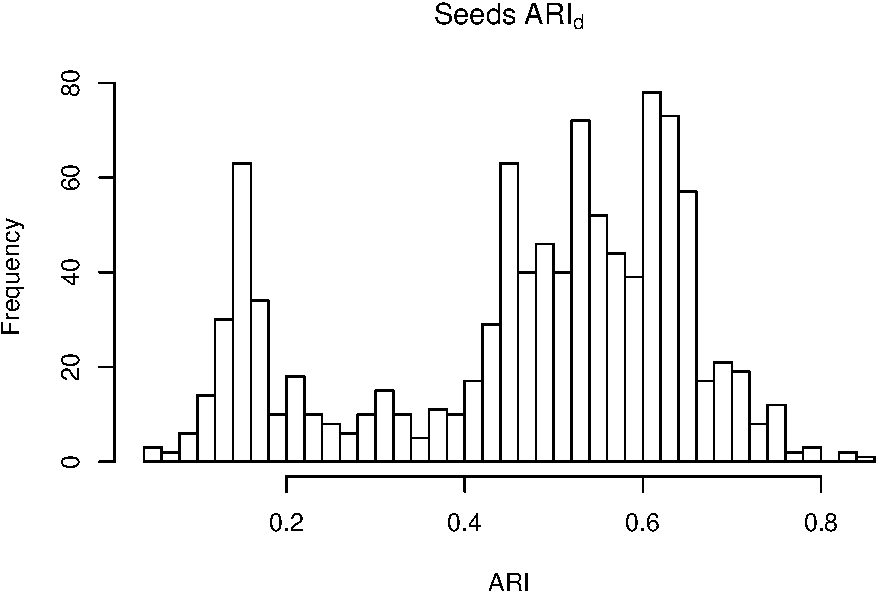
\includegraphics[width=0.7\linewidth]{Report_files/figure-latex/unnamed-chunk-12-5}
\caption{
نمودار فراوانی عملکرد خوشه‌بندی 
$\mathrm{ARI}_d$
پس از کاهش بعد با استفاده از تصویر تصادفی
کوشی (%
$\alpha=1$%
)
به 
سه (%
$d=3$%
)
بعد برای مجموعه داده‌های
بذر
\ref{sec:Seeds}
این نمودار فراوانی،
قله‌های
مشخصی را نشان 
می‌دهد
و مقادیر آن طیف 
محدودی
را پوشش می‌دهند.
}
\end{figure}

\begin{figure}[H]
\centering
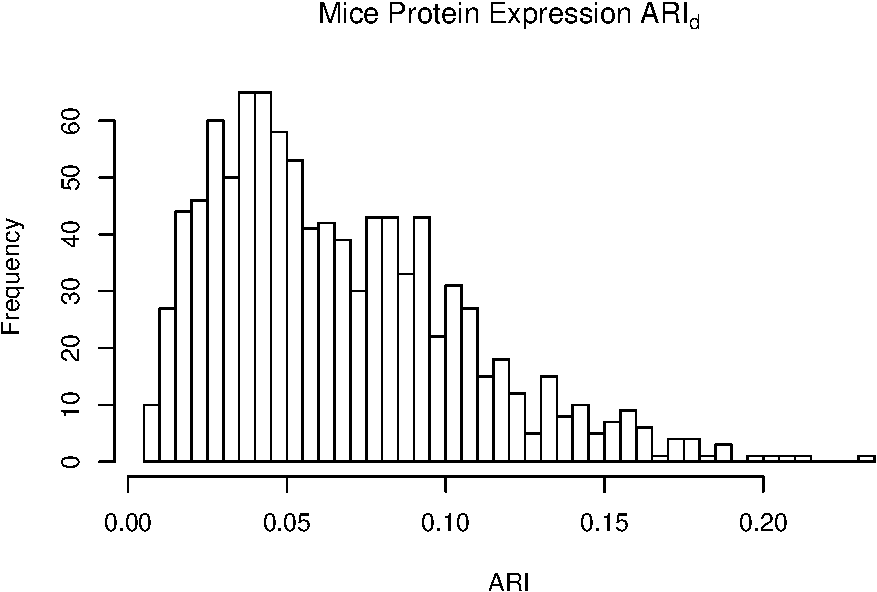
\includegraphics[width=0.7\linewidth]{Report_files/figure-latex/unnamed-chunk-12-6}
\caption{
نمودار فراوانی عملکرد خوشه‌بندی 
$\mathrm{ARI}_d$
پس از کاهش بعد با استفاده از تصویر تصادفی
کوشی (%
$\alpha=1$%
)
به
سه (%
$d=3$%
)
بعد برای مجموعه داده‌های
پروتئین
\ref{sec:MPE}
این نمودار فراوانی،
قله
مشخصی را نشان 
می‌دهد
و مقادیر آن طیف 
محدودی
 را پوشش می‌دهند.
}
\end{figure}

\begin{figure}[H]
\centering
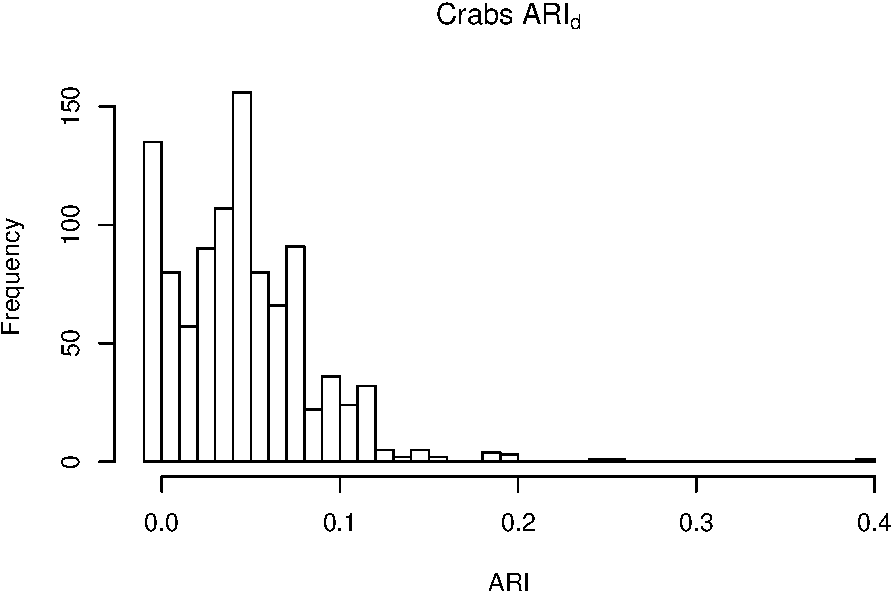
\includegraphics[width=0.7\linewidth]{Report_files/figure-latex/unnamed-chunk-12-7}
\caption{
نمودار فراوانی عملکرد خوشه‌بندی 
$\mathrm{ARI}_d$
پس از کاهش بعد با استفاده از تصویر تصادفی
کوشی (%
$\alpha=1$%
)
به
سه (%
$d=3$%
)
بعد برای مجموعه داده‌های
خرچنگ
\ref{sec:Crabs}
این نمودار فراوانی،
قله
مشخصی را نشان 
می‌دهد
و مقادیر آن طیف 
محدودی
 را پوشش می‌دهند.
}
\end{figure}


\section{
نتایج برای کاهش بعد گسسته $s=2$ به دو بعد
}
\label{sec:S2D2}

\subsection{جداول مقایسه عملکرد خوشه‌بندی}

\begin{table}[H]
\caption{
عملکرد تصویر تصادفی گسسته با
$s=2$
برای کاهش بعد به دو بعد
}
\centering\rowcolors{2}{gray!6}{white}
\begin{latin}
\begin{tabular}{lrrr}
\hiderowcolors
\toprule
Dataset & $ARI_p$ & $ARI_d$ & $C_e$\\
\midrule
\showrowcolors
Thyroid & 0.5831656 & 0.4016237 & -18\\
Iris & 0.6201352 & 0.4890477 & -13\\
Diabetes & 0.3801662 & 0.3515435 & -3\\
Swiss Banknotes & 0.8456292 & 0.4012454 & -44\\
Seeds & 0.7732937 & 0.4459104 & -33\\
\addlinespace
Mice Protein Expression & 0.1314435 & 0.0647088 & -7\\
Crabs & 0.0481402 & 0.0467305 & 0\\
\bottomrule
\end{tabular}
\end{latin}
\rowcolors{2}{white}{white}
\end{table}

\subsection{نمودار فراوانی عملکرد خوشه‌بندی}


\begin{figure}[H]
\centering
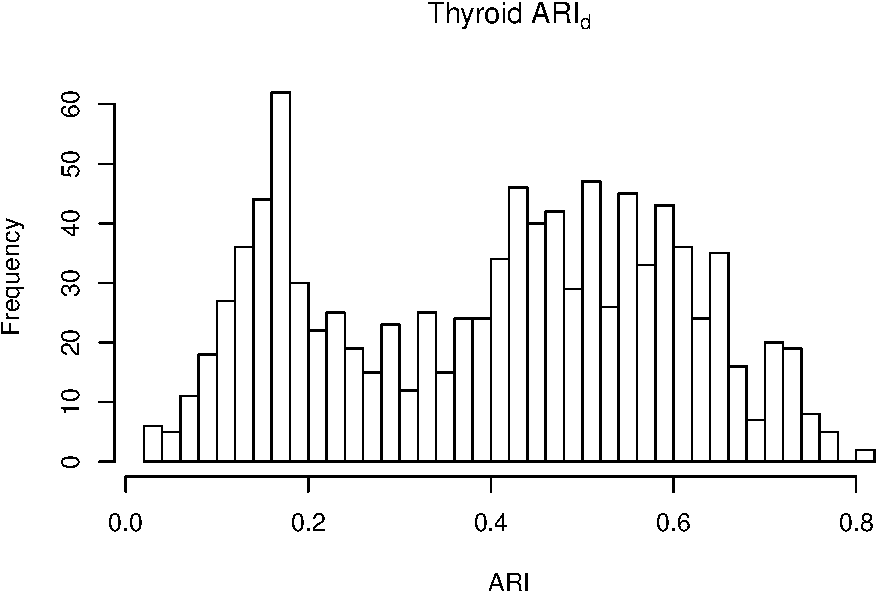
\includegraphics[width=0.7\linewidth]{Report_files/figure-latex/unnamed-chunk-15-1}
\caption{
نمودار فراوانی عملکرد خوشه‌بندی 
$\mathrm{ARI}_d$
پس از کاهش بعد با استفاده از تصویر تصادفی
گسسته (%
$s=2$%
)
به دو (%
$d=2$%
)
بعد برای مجموعه داده‌های
تیروئید
\ref{sec:Thyroid}
این نمودار فراوانی،
قله‌های
مشخصی را نشان 
می‌دهد
و مقادیر آن طیف 
وسیعی را پوشش می‌دهند.
}
\end{figure}

\begin{figure}[H]
\centering
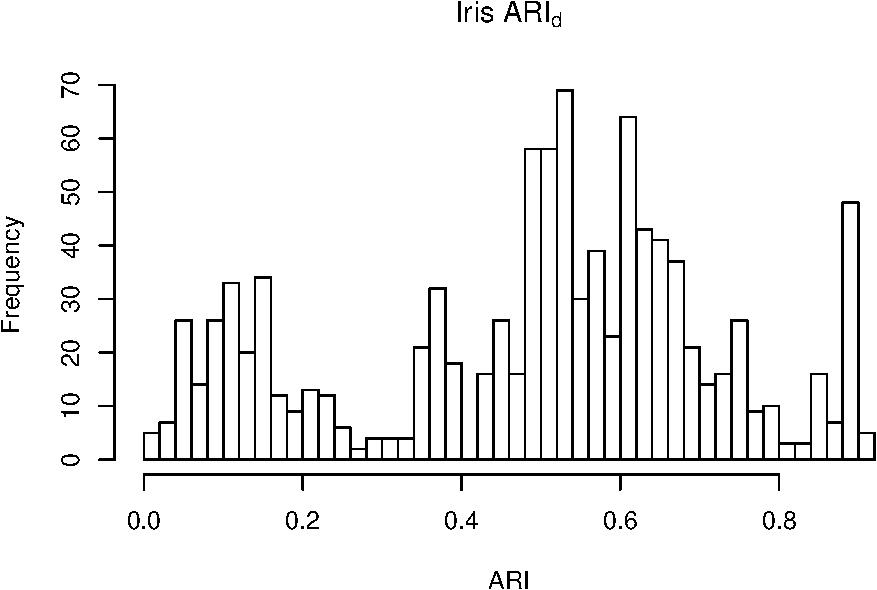
\includegraphics[width=0.7\linewidth]{Report_files/figure-latex/unnamed-chunk-15-2}
\caption{
نمودار فراوانی عملکرد خوشه‌بندی 
$\mathrm{ARI}_d$
پس از کاهش بعد با استفاده از تصویر تصادفی
گسسته (%
$s=2$%
)
به دو (%
$d=2$%
)
بعد برای مجموعه داده‌های
آیریس
\ref{sec:Iris}
این نمودار فراوانی،
قله‌های
مشخصی را نشان 
می‌دهد
و مقادیر آن طیف 
وسیعی را پوشش می‌دهند.
}
\end{figure}

\begin{figure}[H]
\centering
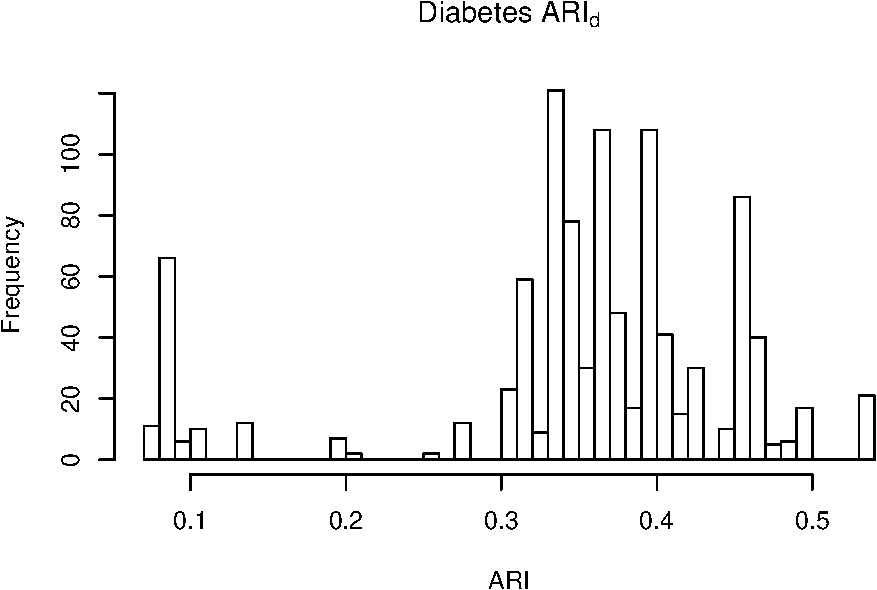
\includegraphics[width=0.7\linewidth]{Report_files/figure-latex/unnamed-chunk-15-3}
\caption{
نمودار فراوانی عملکرد خوشه‌بندی 
$\mathrm{ARI}_d$
پس از کاهش بعد با استفاده از تصویر تصادفی
گسسته (%
$s=2$%
)
به دو (%
$d=2$%
)
بعد برای مجموعه داده‌های
دیابت
\ref{sec:Diabetes}
این نمودار فراوانی،
قله‌های
مشخصی را نشان 
می‌دهد
و مقادیر آن طیف 
محدودی
 را پوشش می‌دهند.
}
\end{figure}

\begin{figure}[H]
\centering
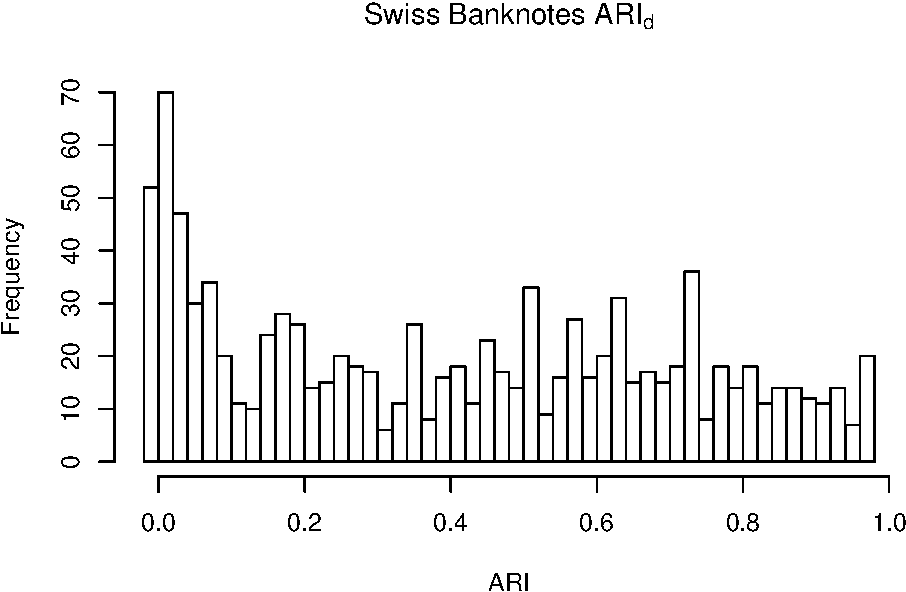
\includegraphics[width=0.7\linewidth]{Report_files/figure-latex/unnamed-chunk-15-4}
\caption{
نمودار فراوانی عملکرد خوشه‌بندی 
$\mathrm{ARI}_d$
پس از کاهش بعد با استفاده از تصویر تصادفی
گسسته (%
$s=2$%
)
به دو (%
$d=2$%
)
بعد برای مجموعه داده‌های
اسکناس
\ref{sec:Swiss}
این نمودار فراوانی،
قله
مشخصی را نشان 
نمی‌دهد
و مقادیر آن طیف 
وسیعی را پوشش می‌دهند.
}
\end{figure}

\begin{figure}[H]
\centering
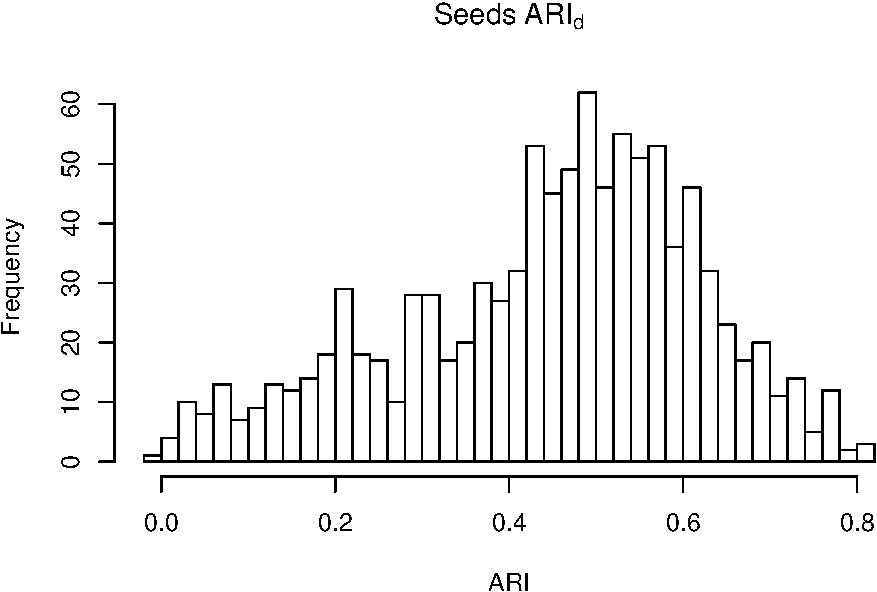
\includegraphics[width=0.7\linewidth]{Report_files/figure-latex/unnamed-chunk-15-5}
\caption{
نمودار فراوانی عملکرد خوشه‌بندی 
$\mathrm{ARI}_d$
پس از کاهش بعد با استفاده از تصویر تصادفی
گسسته (%
$s=2$%
)
به دو (%
$d=2$%
)
بعد برای مجموعه داده‌های
بذر
\ref{sec:Seeds}
این نمودار فراوانی،
قله
مشخصی را نشان 
می‌دهد
و مقادیر آن طیف 
محدودی
 را پوشش می‌دهند.
}
\end{figure}

\begin{figure}[H]
\centering
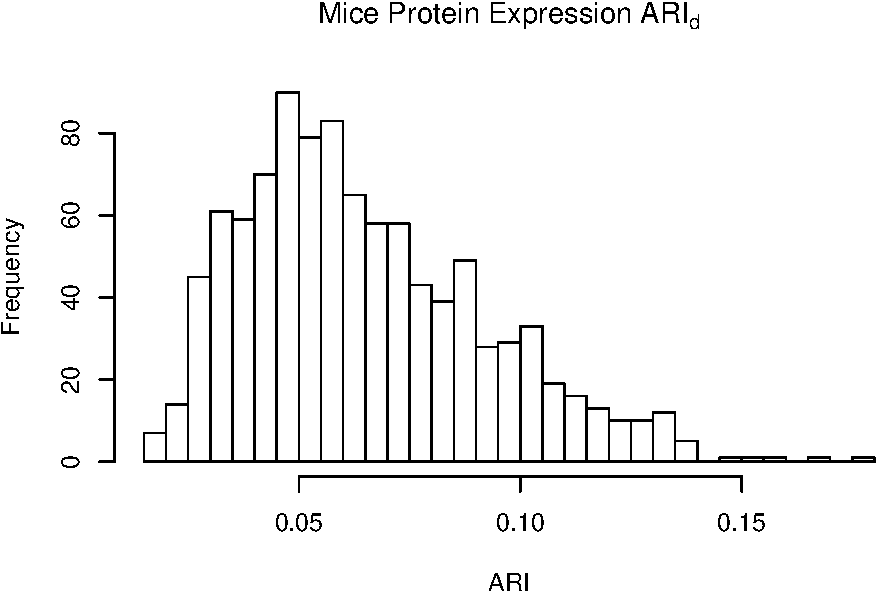
\includegraphics[width=0.7\linewidth]{Report_files/figure-latex/unnamed-chunk-15-6}
\caption{
نمودار فراوانی عملکرد خوشه‌بندی 
$\mathrm{ARI}_d$
پس از کاهش بعد با استفاده از تصویر تصادفی
گسسته (%
$s=2$%
)
به دو (%
$d=2$%
)
بعد برای مجموعه داده‌های
پروتئین
\ref{sec:MPE}
این نمودار فراوانی،
قله
مشخصی را نشان 
می‌دهد
و مقادیر آن طیف 
محدودی
 را پوشش می‌دهند.
}
\end{figure}

\begin{figure}[H]
\centering
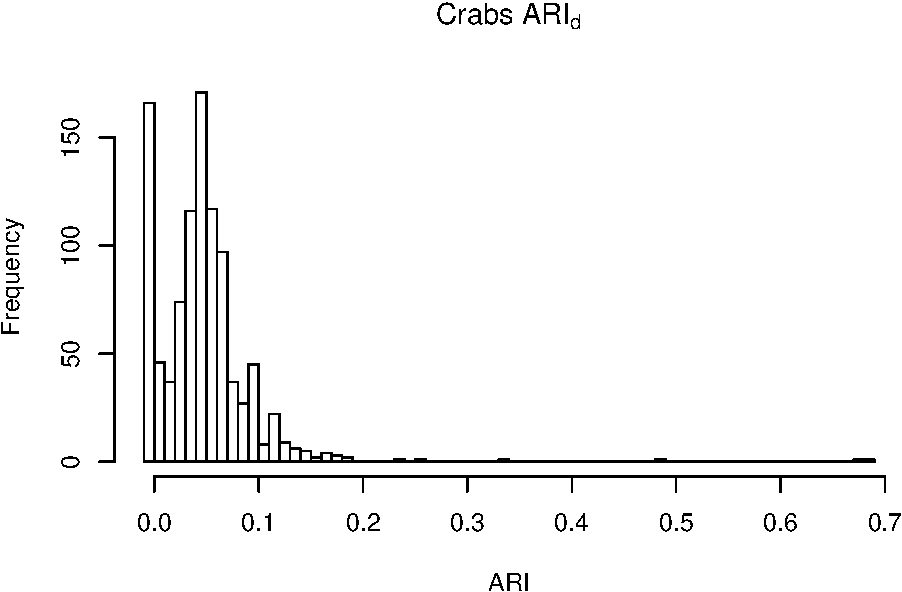
\includegraphics[width=0.7\linewidth]{Report_files/figure-latex/unnamed-chunk-15-7}
\caption{
نمودار فراوانی عملکرد خوشه‌بندی 
$\mathrm{ARI}_d$
پس از کاهش بعد با استفاده از تصویر تصادفی
گسسته (%
$s=2$%
)
به دو (%
$d=2$%
)
بعد برای مجموعه داده‌های
خرچنگ
\ref{sec:Crabs}
این نمودار فراوانی،
قله
مشخصی را نشان 
می‌دهد
و مقادیر آن طیف 
محدودی
 را پوشش می‌دهند.
}
\end{figure}


\section{
نتایج برای کاهش بعد گسسته $s=2$ به سه بعد
}
\label{sec:S2D3}

\subsection{جداول مقایسه عملکرد خوشه‌بندی}

\begin{table}[H]
\caption{
عملکرد تصویر تصادفی گسسته با 
$s=2$
برای کاهش بعد به سه بعد
}
\centering\rowcolors{2}{gray!6}{white}
\begin{latin}
\begin{tabular}{lrrr}
\hiderowcolors
\toprule
Dataset & $ARI_p$ & $ARI_d$ & $C_e$\\
\midrule
\showrowcolors
Thyroid & 0.5831656 & 0.4386178 & -14\\
Iris & 0.6201352 & 0.5410759 & -8\\
Swiss Banknotes & 0.8456292 & 0.4881694 & -36\\
Seeds & 0.7732937 & 0.5289697 & -24\\
\addlinespace
Mice Protein Expression & 0.1314406 & 0.0798832 & -5\\
Crabs & 0.0481402 & 0.0463655 & 0\\
\bottomrule
\end{tabular}
\end{latin}
\rowcolors{2}{white}{white}
\end{table}


\subsection{نمودار فراوانی عملکرد خوشه‌بندی}


\begin{figure}[H]
\centering
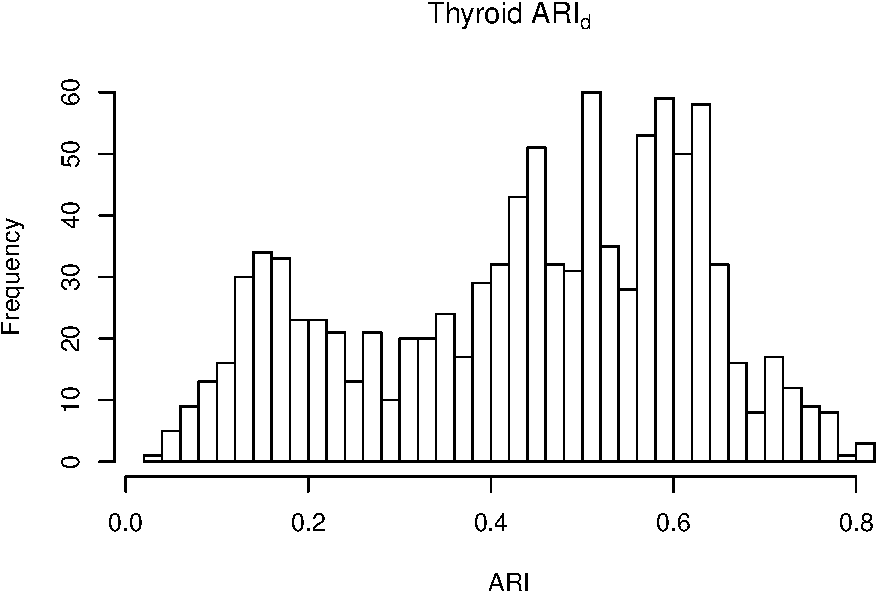
\includegraphics[width=0.7\linewidth]{Report_files/figure-latex/unnamed-chunk-18-1}
\caption{
نمودار فراوانی عملکرد خوشه‌بندی 
$\mathrm{ARI}_d$
پس از کاهش بعد با استفاده از تصویر تصادفی
گسسته (%
$s=2$%
)
به
سه (%
$d=3$%
)
بعد برای مجموعه داده‌های
تیروئید
\ref{sec:Thyroid}
این نمودار فراوانی،
قله
مشخصی را نشان 
نمی‌دهد
و مقادیر آن طیف 
وسیعی را پوشش می‌دهند.
}
\end{figure}

\begin{figure}[H]
\centering
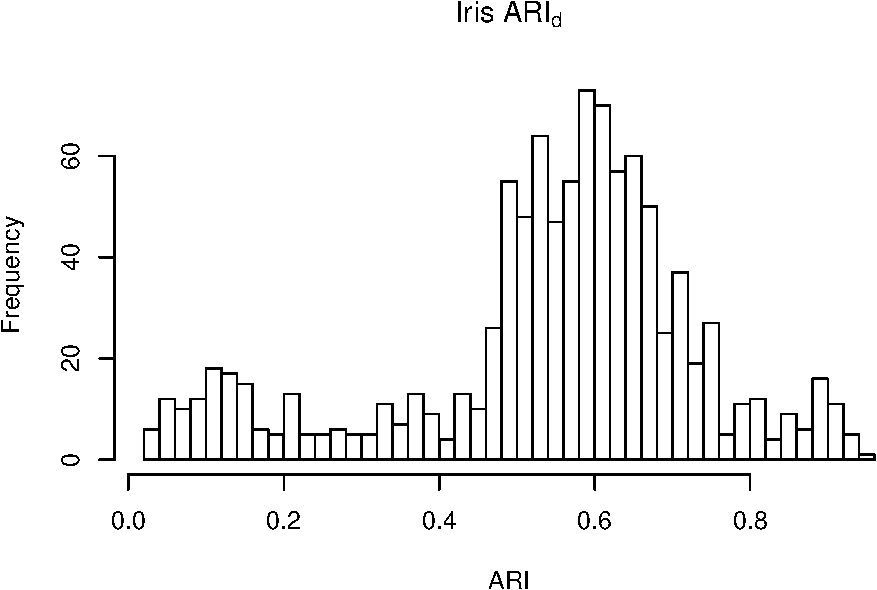
\includegraphics[width=0.7\linewidth]{Report_files/figure-latex/unnamed-chunk-18-2}
\caption{
نمودار فراوانی عملکرد خوشه‌بندی 
$\mathrm{ARI}_d$
پس از کاهش بعد با استفاده از تصویر تصادفی
گسسته (%
$s=2$%
)
به
سه (%
$d=3$%
)
بعد برای مجموعه داده‌های
آیریس
\ref{sec:Iris}
این نمودار فراوانی،
قله
مشخصی را نشان 
می‌دهد
و مقادیر آن طیف 
محدودی
 را پوشش می‌دهند.
}
\end{figure}

\begin{figure}[H]
\centering
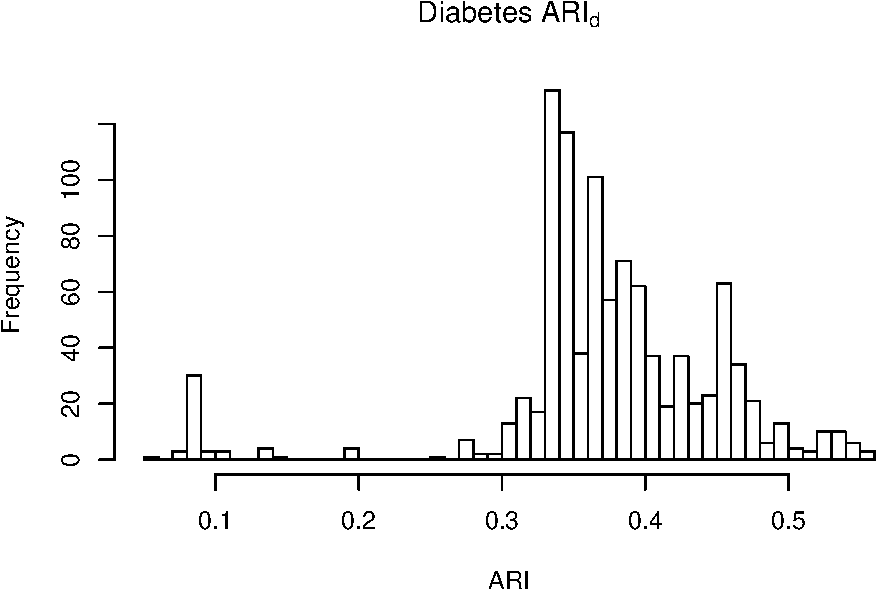
\includegraphics[width=0.7\linewidth]{Report_files/figure-latex/unnamed-chunk-18-3}
\caption{
نمودار فراوانی عملکرد خوشه‌بندی 
$\mathrm{ARI}_d$
پس از کاهش بعد با استفاده از تصویر تصادفی
گسسته (%
$s=2$%
)
به
سه (%
$d=3$%
)
بعد برای مجموعه داده‌های
دیابت
\ref{sec:Diabetes}
این نمودار فراوانی،
قله
مشخصی را نشان 
می‌دهد
و مقادیر آن طیف 
محدودی
 را پوشش می‌دهند.
}
\end{figure}

\begin{figure}[H]
\centering
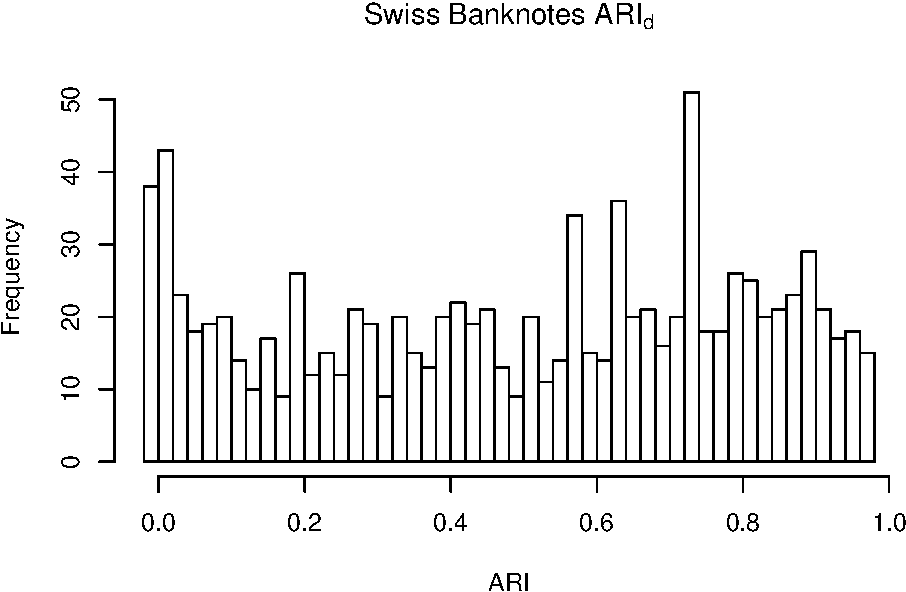
\includegraphics[width=0.7\linewidth]{Report_files/figure-latex/unnamed-chunk-18-4}
\caption{
نمودار فراوانی عملکرد خوشه‌بندی 
$\mathrm{ARI}_d$
پس از کاهش بعد با استفاده از تصویر تصادفی
گسسته (%
$s=2$%
)
به
سه (%
$d=3$%
)
بعد برای مجموعه داده‌های
اسکناس
\ref{sec:Swiss}
این نمودار فراوانی،
قله
مشخصی را نشان 
نمی‌دهد
و مقادیر آن طیف 
وسیعی را پوشش می‌دهند.
}
\end{figure}

\begin{figure}[H]
\centering
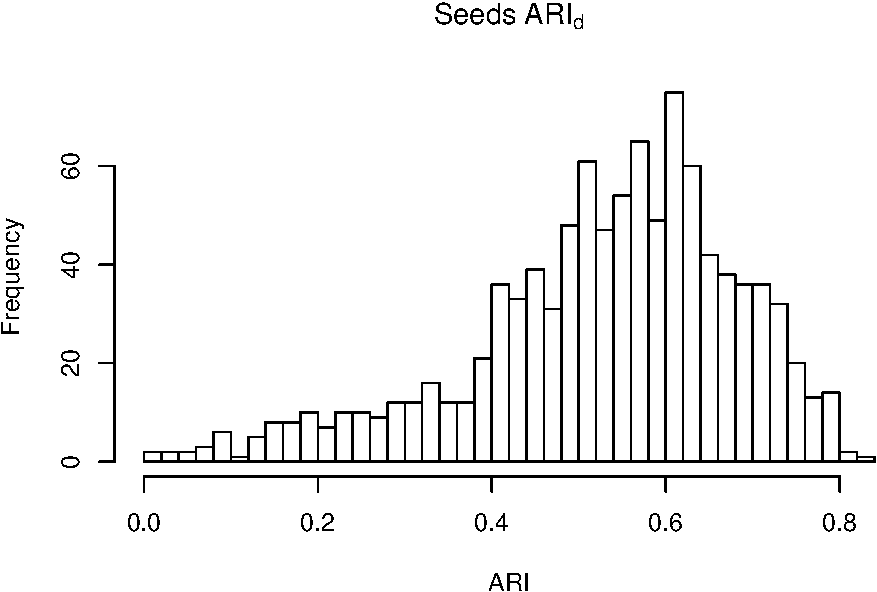
\includegraphics[width=0.7\linewidth]{Report_files/figure-latex/unnamed-chunk-18-5}
\caption{
نمودار فراوانی عملکرد خوشه‌بندی 
$\mathrm{ARI}_d$
پس از کاهش بعد با استفاده از تصویر تصادفی
گسسته (%
$s=2$%
)
به 
سه (%
$d=3$%
)
بعد برای مجموعه داده‌های
بذر
\ref{sec:Seeds}
این نمودار فراوانی،
قله
مشخصی را نشان 
می‌دهد
و مقادیر آن طیف 
محدودی
را پوشش می‌دهند.
}
\end{figure}

\begin{figure}[H]
\centering
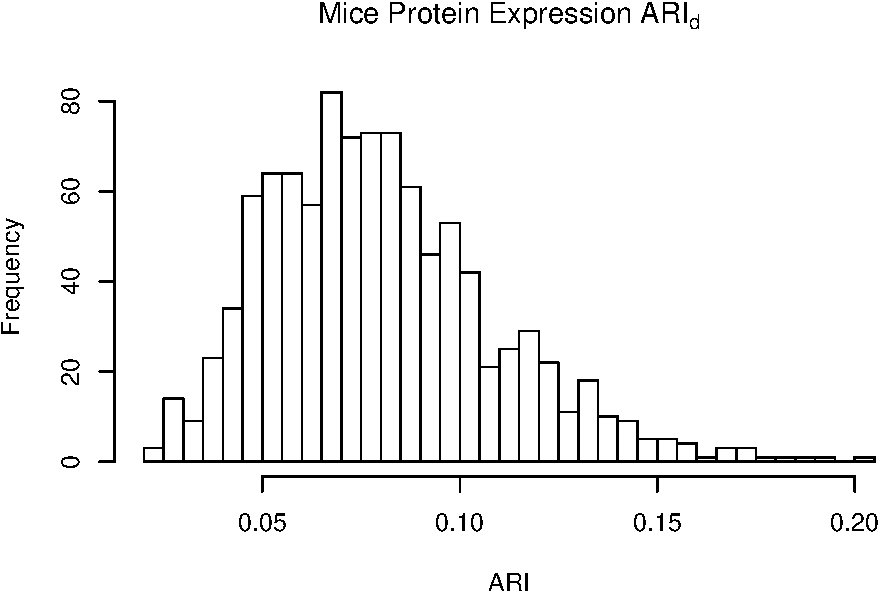
\includegraphics[width=0.7\linewidth]{Report_files/figure-latex/unnamed-chunk-18-6}
\caption{
نمودار فراوانی عملکرد خوشه‌بندی 
$\mathrm{ARI}_d$
پس از کاهش بعد با استفاده از تصویر تصادفی
گسسته (%
$s=2$%
)
به
سه (%
$d=3$%
)
بعد برای مجموعه داده‌های
پروتئین
\ref{sec:MPE}
این نمودار فراوانی،
قله
مشخصی را نشان 
می‌دهد
و مقادیر آن طیف 
محدودی
 را پوشش می‌دهند.
}
\end{figure}

\begin{figure}[H]
\centering
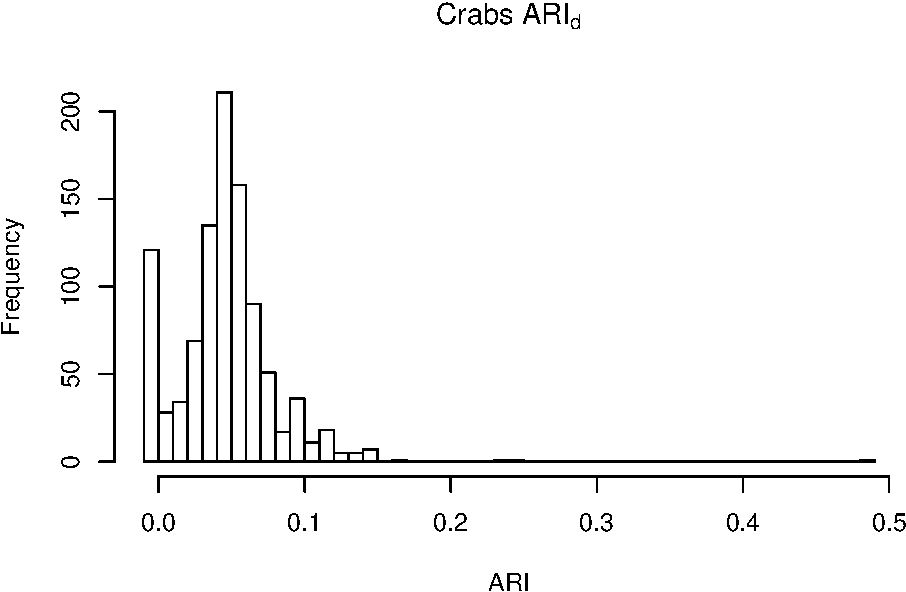
\includegraphics[width=0.7\linewidth]{Report_files/figure-latex/unnamed-chunk-18-7}
\caption{
نمودار فراوانی عملکرد خوشه‌بندی 
$\mathrm{ARI}_d$
پس از کاهش بعد با استفاده از تصویر تصادفی
گسسته (%
$s=2$%
)
به
سه (%
$d=3$%
)
بعد برای مجموعه داده‌های
خرچنگ
\ref{sec:Crabs}
این نمودار فراوانی،
قله
مشخصی را نشان 
می‌دهد
و مقادیر آن طیف 
محدودی
 را پوشش می‌دهند.
}
\end{figure}



\section{
بررسی تابعیت عملکرد کاهش بعد $C_e$ به ازای تغییر $\alpha$ برای کاهش بعد به دو بعد
}


\begin{figure}[H]
\centering
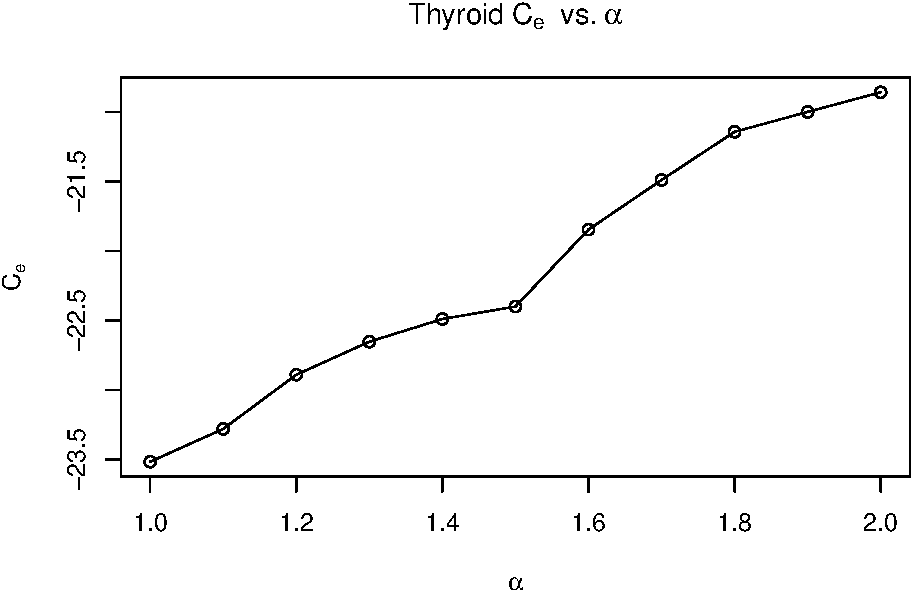
\includegraphics[width=0.7\linewidth]{Report_files/figure-latex/unnamed-chunk-20-1}
\caption{
نمودار تغییرات عملکرد کاهش بعد 
$C_e$
به ازای تغییر پارامتر
$\alpha$
برای کاهش بعد به 
دو
بعد بر روی مجموعه داده‌‌‌ی 
تیروئید
\ref{sec:Thyroid}
. این نمودار بیانگر این است که برای این مجموعه داده کاهش بعد 
نرمال
بهتر از کاهش بعد 
کوشی 
عمل می‌کند
}
\end{figure}


\begin{figure}[H]
\centering
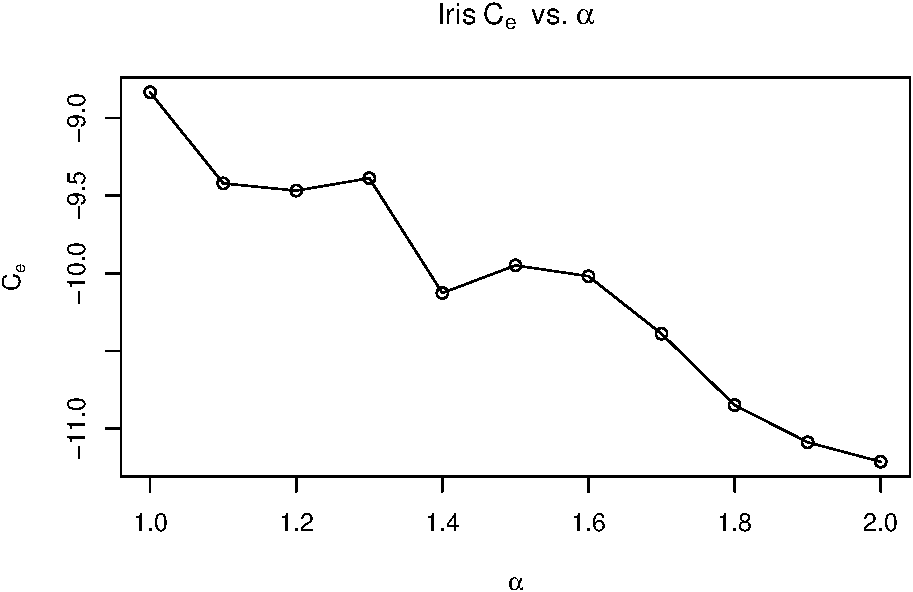
\includegraphics[width=0.7\linewidth]{Report_files/figure-latex/unnamed-chunk-20-2}
\caption{
نمودار تغییرات عملکرد کاهش بعد 
$C_e$
به ازای تغییر پارامتر
$\alpha$
برای کاهش بعد به 
دو
 بعد بر روی مجموعه داده‌‌‌ی 
آیریس
\ref{sec:Iris}
. این نمودار بیانگر این است که برای این مجموعه داده کاهش بعد 
کوشی 
بهتر از کاهش بعد 
نرمال
عمل می‌کند
}
\end{figure}

\begin{figure}[H]
\centering
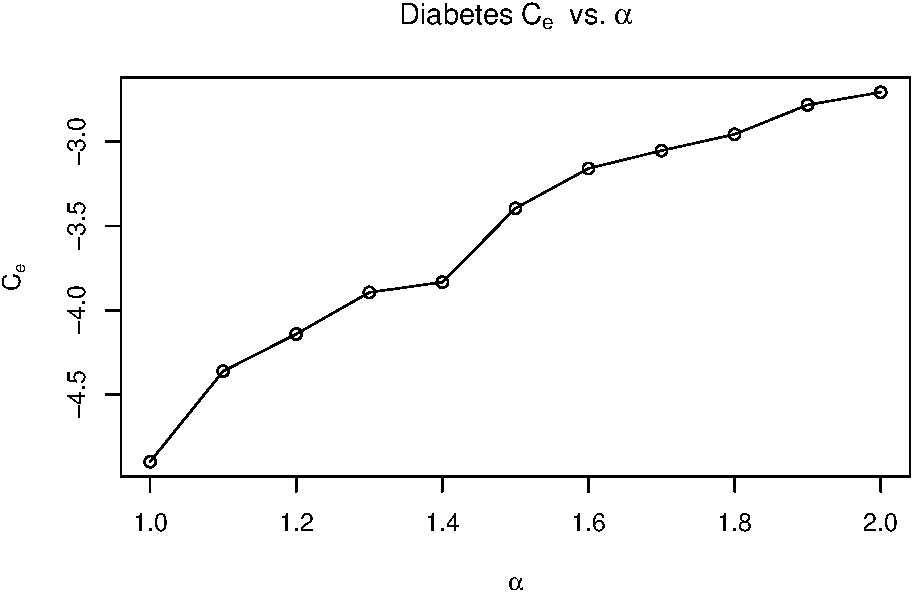
\includegraphics[width=0.7\linewidth]{Report_files/figure-latex/unnamed-chunk-20-3}
\caption{
نمودار تغییرات عملکرد کاهش بعد 
$C_e$
به ازای تغییر پارامتر
$\alpha$
برای کاهش بعد به 
دو
 بعد بر روی مجموعه داده‌‌‌ی 
دیابت
\ref{sec:Diabetes}
. این نمودار بیانگر این است که برای این مجموعه داده کاهش بعد 
نرمال
بهتر از کاهش بعد 
کوشی 
عمل می‌کند
}
\end{figure}

\begin{figure}[H]
\centering
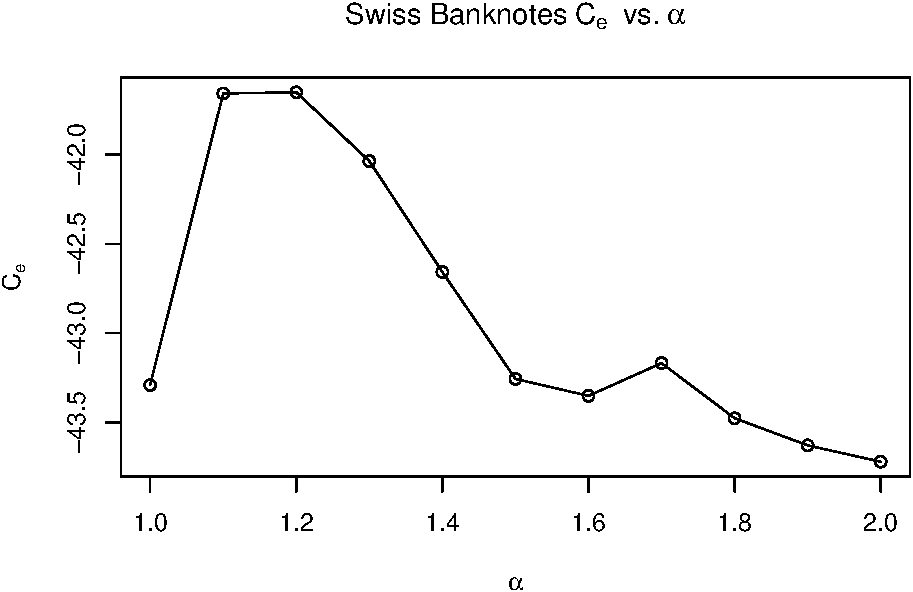
\includegraphics[width=0.7\linewidth]{Report_files/figure-latex/unnamed-chunk-20-4}
\caption{
نمودار تغییرات عملکرد کاهش بعد 
$C_e$
به ازای تغییر پارامتر
$\alpha$
برای کاهش بعد به 
دو
بعد بر روی مجموعه داده‌‌‌ی 
اسکناس
\ref{sec:Swiss}
. این نمودار بیانگر این است که برای این مجموعه داده کاهش بعد 
نزدیک به 
کوشی 
بهتر از کاهش بعد 
کوشی و نرمال
عمل می‌کند
}
\end{figure}

\begin{figure}[H]
\centering
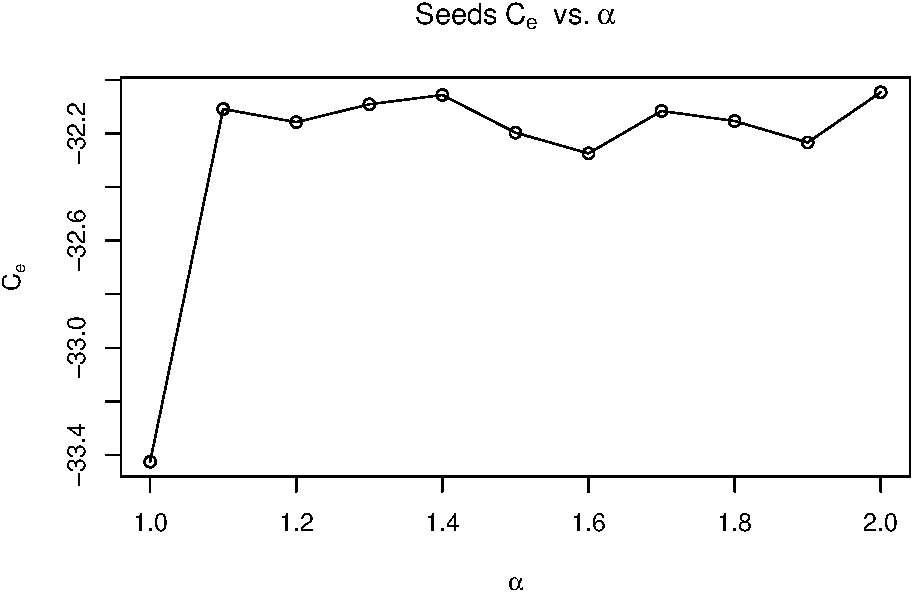
\includegraphics[width=0.7\linewidth]{Report_files/figure-latex/unnamed-chunk-20-5}
\caption{
نمودار تغییرات عملکرد کاهش بعد 
$C_e$
به ازای تغییر پارامتر
$\alpha$
برای کاهش بعد به 
دو
 بعد بر روی مجموعه داده‌‌‌ی 
بذر
\ref{sec:Seeds}
. این نمودار بیانگر این است که برای این مجموعه داده کاهش بعد 
کوشی خوب
عمل نمی‌کند
}
\end{figure}

\begin{figure}[H]
\centering
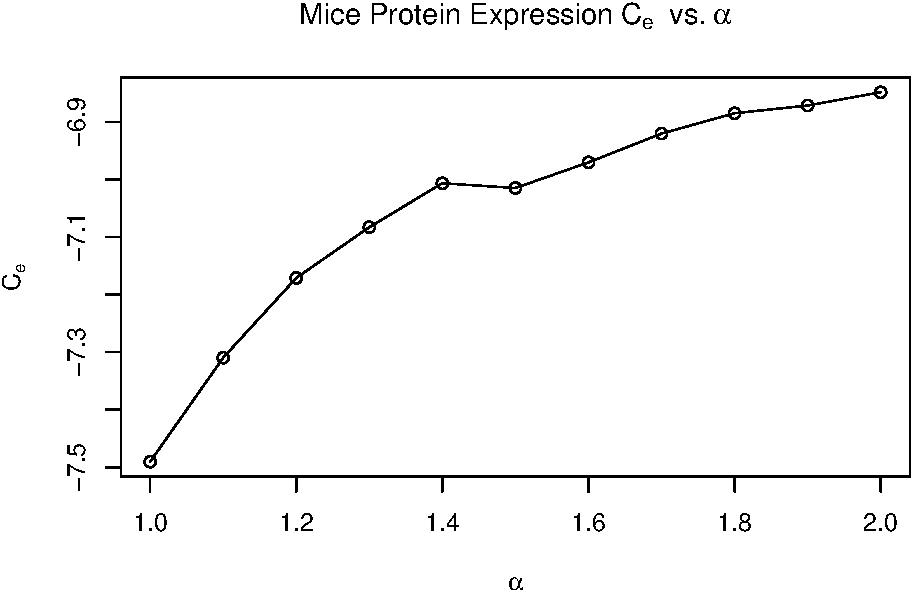
\includegraphics[width=0.7\linewidth]{Report_files/figure-latex/unnamed-chunk-20-6}
\caption{
نمودار تغییرات عملکرد کاهش بعد 
$C_e$
به ازای تغییر پارامتر
$\alpha$
برای کاهش بعد به 
دو
 بعد بر روی مجموعه داده‌‌‌ی 
پروتئین
\ref{sec:MPE}
. این نمودار بیانگر این است که برای این مجموعه داده کاهش بعد 
نرمال
بهتر از کاهش بعد 
کوشی 
عمل می‌کند
}
\end{figure}

\begin{figure}[H]
\centering
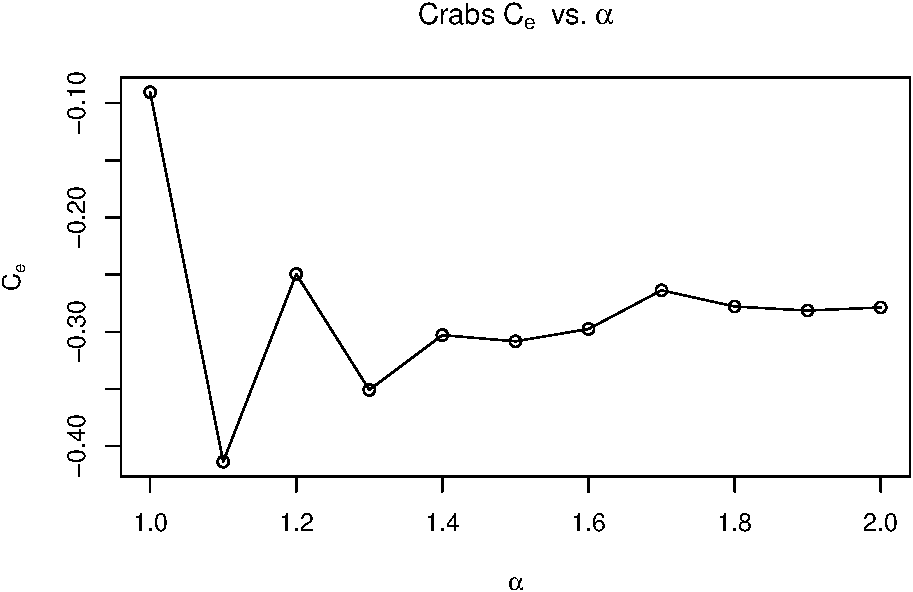
\includegraphics[width=0.7\linewidth]{Report_files/figure-latex/unnamed-chunk-20-7}
\caption{
نمودار تغییرات عملکرد کاهش بعد 
$C_e$
به ازای تغییر پارامتر
$\alpha$
برای کاهش بعد به 
دو
بعد بر روی مجموعه داده‌‌‌ی 
خرچنگ
\ref{sec:Crabs}
. این نمودار بیانگر این است که برای این مجموعه داده کاهش بعد 
تفاوت خاصی میان عملکرد کاهش بعد نرمال تا کوشی وجود ندارد
}
\end{figure}



\section{
بررسی تابعیت عملکرد کاهش بعد $C_e$ به ازای تغییر $\alpha$ برای کاهش بعد به سه بعد
}


\begin{figure}[H]
\centering
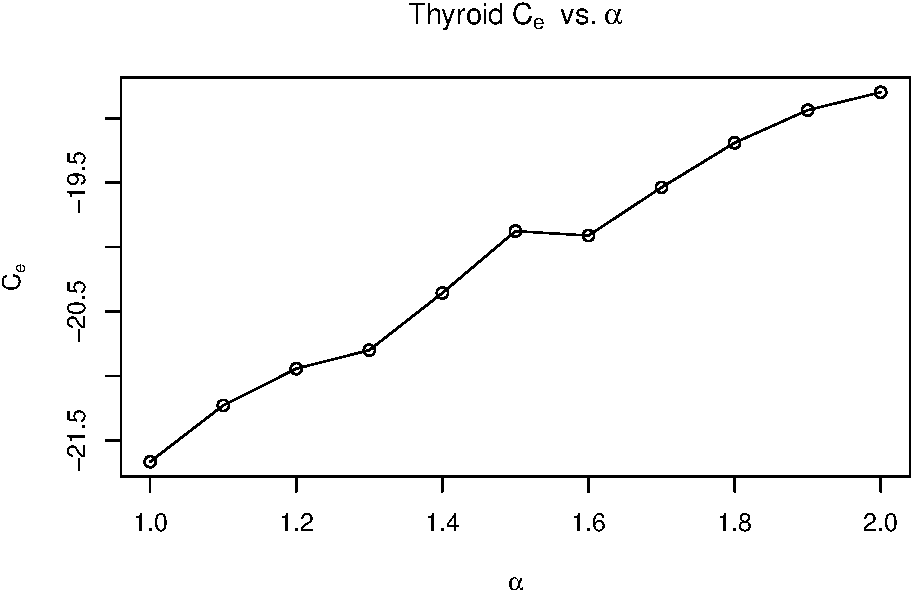
\includegraphics[width=0.7\linewidth]{Report_files/figure-latex/unnamed-chunk-22-1}
\caption{
نمودار تغییرات عملکرد کاهش بعد 
$C_e$
به ازای تغییر پارامتر
$\alpha$
برای کاهش بعد به 
سه بعد بر روی مجموعه داده‌‌‌ی 
تیروئید
\ref{sec:Thyroid}
. این نمودار بیانگر این است که برای این مجموعه داده کاهش بعد 
نرمال
اندکی بهتر از کاهش بعد 
کوشی 
عمل می‌کند
}
\end{figure}

\begin{figure}[H]
\centering
\includegraphics[width=0.7\linewidth]{Report_files/figure-latex/unnamed-chunk-22-2}
\caption{
نمودار تغییرات عملکرد کاهش بعد 
$C_e$
به ازای تغییر پارامتر
$\alpha$
برای کاهش بعد به 
سه بعد بر روی مجموعه داده‌‌‌ی 
آیریس
\ref{sec:Iris}
. این نمودار بیانگر این است که برای این مجموعه داده کاهش بعد 
کوشی 
خوب عمل نمی‌کند
}
\end{figure}

\begin{figure}[H]
\centering
\includegraphics[width=0.7\linewidth]{Report_files/figure-latex/unnamed-chunk-22-3}
\caption{
نمودار تغییرات عملکرد کاهش بعد 
$C_e$
به ازای تغییر پارامتر
$\alpha$
برای کاهش بعد به 
سه بعد بر روی مجموعه داده‌‌‌ی 
دیابت
\ref{sec:Diabetes}
. این نمودار بیانگر این است که برای این مجموعه داده کاهش بعد 
نرمال
بهتر از کاهش بعد 
کوشی 
عمل می‌کند
}
\end{figure}

\begin{figure}[H]
\centering
\includegraphics[width=0.7\linewidth]{Report_files/figure-latex/unnamed-chunk-22-4}
\caption{
نمودار تغییرات عملکرد کاهش بعد 
$C_e$
به ازای تغییر پارامتر
$\alpha$
برای کاهش بعد به 
سه بعد بر روی مجموعه داده‌‌‌ی 
اسکناس
\ref{sec:Swiss}
. این نمودار بیانگر این است که برای این مجموعه داده کاهش بعد 
کوشی 
بهتر از کاهش بعد 
نرمال
عمل می‌کند
}
\end{figure}

\begin{figure}[H]
\centering
\includegraphics[width=0.7\linewidth]{Report_files/figure-latex/unnamed-chunk-22-5}
\caption{
نمودار تغییرات عملکرد کاهش بعد 
$C_e$
به ازای تغییر پارامتر
$\alpha$
برای کاهش بعد به 
سه بعد بر روی مجموعه داده‌‌‌ی 
بذر
\ref{sec:Seeds}
. این نمودار بیانگر این است که برای این مجموعه داده کاهش بعد 
نرمال
بهتر از کاهش بعد 
کوشی 
عمل می‌کند
}
\end{figure}

\begin{figure}[H]
\centering
\includegraphics[width=0.7\linewidth]{Report_files/figure-latex/unnamed-chunk-22-6}
\caption{
نمودار تغییرات عملکرد کاهش بعد 
$C_e$
به ازای تغییر پارامتر
$\alpha$
برای کاهش بعد به 
سه بعد بر روی مجموعه داده‌‌‌ی 
پروتئین
\ref{sec:MPE}
. این نمودار بیانگر این است که برای این مجموعه داده کاهش بعد 
نرمال
بهتر از کاهش بعد 
کوشی 
عمل می‌کند
}
\end{figure}

\begin{figure}[H]
\centering
\includegraphics[width=0.7\linewidth]{Report_files/figure-latex/unnamed-chunk-22-7}
\caption{
نمودار تغییرات عملکرد کاهش بعد 
$C_e$
به ازای تغییر پارامتر
$\alpha$
برای کاهش بعد به 
سه بعد بر روی مجموعه داده‌‌‌ی 
خرچنگ
\ref{sec:Crabs}
. این نمودار بیانگر این است که برای این مجموعه داده کاهش بعد 
تفاوت خاصی میان عملکرد کاهش بعد نرمال تا کوشی وجود ندارد
}
\end{figure}

\section{
بررسی تابعیت عملکرد کاهش بعد $C_e$ به ازای تغییر $s$ برای کاهش بعد گسسته به دو بعد
}


\begin{figure}[H]
\centering
\includegraphics[width=0.7\linewidth]{Report_files/figure-latex/unnamed-chunk-24-1}
\caption{
نمودار تغییرات عملکرد کاهش بعد 
$C_e$
به ازای تغییر پارامتر
$s$
برای کاهش بعد به 
دو
بعد بر روی مجموعه داده‌‌‌ی 
تیروئید
\ref{sec:Thyroid}
. این نمودار بیانگر این است که برای این مجموعه داده کاهش بعد 
با تصویر تنک‌تر عملکرد کاهش بعد بدتر می‌شود
}
\end{figure}

\begin{figure}[H]
\centering
\includegraphics[width=0.7\linewidth]{Report_files/figure-latex/unnamed-chunk-24-2}
\caption{
نمودار تغییرات عملکرد کاهش بعد 
$C_e$
به ازای تغییر پارامتر
$s$
برای کاهش بعد به 
دو
 بعد بر روی مجموعه داده‌‌‌ی 
آیریس
\ref{sec:Iris}
. این نمودار بیانگر این است که برای این مجموعه داده کاهش بعد 
با تصویر تنک‌تر عملکر کاهش بعد به طرز محسوس تغییر نمی‌کند
}
\end{figure}

\begin{figure}[H]
\centering
\includegraphics[width=0.7\linewidth]{Report_files/figure-latex/unnamed-chunk-24-3}
\caption{
نمودار تغییرات عملکرد کاهش بعد 
$C_e$
به ازای تغییر پارامتر
$s$
برای کاهش بعد به 
دو
 بعد بر روی مجموعه داده‌‌‌ی 
دیابت
\ref{sec:Diabetes}
. این نمودار بیانگر این است که برای این مجموعه داده کاهش بعد 
با تصویر تنک‌تر عملکرد کاهش بعد به شدت بد می‌شود
}
\end{figure}

\begin{figure}[H]
\centering
\includegraphics[width=0.7\linewidth]{Report_files/figure-latex/unnamed-chunk-24-4}
\caption{
نمودار تغییرات عملکرد کاهش بعد 
$C_e$
به ازای تغییر پارامتر
$s$
برای کاهش بعد به 
دو
بعد بر روی مجموعه داده‌‌‌ی 
اسکناس
\ref{sec:Swiss}
. این نمودار بیانگر این است که برای این مجموعه داده کاهش بعد 
با تصویر تنک‌تر عملکرد کاهش بعد به شدت بد می‌شود
}
\end{figure}

\begin{figure}[H]
\centering
\includegraphics[width=0.7\linewidth]{Report_files/figure-latex/unnamed-chunk-24-5}
\caption{
نمودار تغییرات عملکرد کاهش بعد 
$C_e$
به ازای تغییر پارامتر
$s$
برای کاهش بعد به 
دو
بعد بر روی مجموعه داده‌‌‌ی 
بذر
\ref{sec:Seeds}
. این نمودار بیانگر این است که برای این مجموعه داده کاهش بعد 
با تصویر تنک‌تر عملکر کاهش بعد به طرز محسوس تغییر نمی‌کند
}
\end{figure}

\begin{figure}[H]
\centering
\includegraphics[width=0.7\linewidth]{Report_files/figure-latex/unnamed-chunk-24-6}
\caption{
نمودار تغییرات عملکرد کاهش بعد 
$C_e$
به ازای تغییر پارامتر
$s$
برای کاهش بعد به 
دو
 بعد بر روی مجموعه داده‌‌‌ی 
پروتئین
\ref{sec:MPE}
. این نمودار بیانگر این است که برای این مجموعه داده کاهش بعد 
با تصویر تنک‌تر عملکر کاهش بعد به طرز محسوس تغییر نمی‌کند
}
\end{figure}

\begin{figure}[H]
\centering
\includegraphics[width=0.7\linewidth]{Report_files/figure-latex/unnamed-chunk-24-7}
\caption{
نمودار تغییرات عملکرد کاهش بعد 
$C_e$
به ازای تغییر پارامتر
$s$
برای کاهش بعد به 
دو
 بعد بر روی مجموعه داده‌‌‌ی 
خرچنگ
\ref{sec:Crabs}
. این نمودار بیانگر این است که برای این مجموعه داده کاهش بعد 
با تصویر تنک‌تر عملکر کاهش بعد به طرز محسوس تغییر نمی‌کند
}
\end{figure}


\section{
بررسی تابعیت عملکرد کاهش بعد $C_e$ به ازای تغییر $s$ برای کاهش بعد گسسته به سه بعد
}


\begin{figure}[H]
\centering
\includegraphics[width=0.7\linewidth]{Report_files/figure-latex/unnamed-chunk-26-1}
\caption{
نمودار تغییرات عملکرد کاهش بعد 
$C_e$
به ازای تغییر پارامتر
$s$
برای کاهش بعد به 
سه بعد بر روی مجموعه داده‌‌‌ی 
تیروئید
\ref{sec:Thyroid}
. این نمودار بیانگر این است که برای این مجموعه داده کاهش بعد 
با تصویر تنک‌تر عملکرد کاهش بعد به شدت بد می‌شود
}
\end{figure}

\begin{figure}[H]
\centering
\includegraphics[width=0.7\linewidth]{Report_files/figure-latex/unnamed-chunk-26-2}
\caption{
نمودار تغییرات عملکرد کاهش بعد 
$C_e$
به ازای تغییر پارامتر
$s$
برای کاهش بعد به 
سه بعد بر روی مجموعه داده‌‌‌ی 
آیریس
\ref{sec:Iris}
. این نمودار بیانگر این است که برای این مجموعه داده کاهش بعد 
با تصویر تنک‌تر عملکرد کاهش بعد به شدت بد می‌شود
}
\end{figure}

\begin{figure}[H]
\centering
\includegraphics[width=0.7\linewidth]{Report_files/figure-latex/unnamed-chunk-26-3}
\caption{
نمودار تغییرات عملکرد کاهش بعد 
$C_e$
به ازای تغییر پارامتر
$s$
برای کاهش بعد به 
سه بعد بر روی مجموعه داده‌‌‌ی 
دیابت
\ref{sec:Diabetes}
. این نمودار بیانگر این است که برای این مجموعه داده کاهش بعد 
با تصویر تنک‌ مشخص با 
$s=1.7$
 عملکرد بهتری دارد
}
\end{figure}

\begin{figure}[H]
\centering
\includegraphics[width=0.7\linewidth]{Report_files/figure-latex/unnamed-chunk-26-4}
\caption{
نمودار تغییرات عملکرد کاهش بعد 
$C_e$
به ازای تغییر پارامتر
$s$
برای کاهش بعد به 
سه بعد بر روی مجموعه داده‌‌‌ی 
اسکناس
\ref{sec:Swiss}
. این نمودار بیانگر این است که برای این مجموعه داده کاهش بعد 
با تصویر تنک‌تر عملکرد کاهش بعد به شدت بد می‌شود
}
\end{figure}

\begin{figure}[H]
\centering
\includegraphics[width=0.7\linewidth]{Report_files/figure-latex/unnamed-chunk-26-5}
\caption{
نمودار تغییرات عملکرد کاهش بعد 
$C_e$
به ازای تغییر پارامتر
$s$
برای کاهش بعد به 
سه بعد بر روی مجموعه داده‌‌‌ی 
بذر
\ref{sec:Seeds}
. این نمودار بیانگر این است که برای این مجموعه داده کاهش بعد 
با تصویر تنک‌ مشخص با 
$s=1.8$
 عملکرد کاهش بعد بهتر است
}
\end{figure}

\begin{figure}[H]
\centering
\includegraphics[width=0.7\linewidth]{Report_files/figure-latex/unnamed-chunk-26-6}
\caption{
نمودار تغییرات عملکرد کاهش بعد 
$C_e$
به ازای تغییر پارامتر
$s$
برای کاهش بعد به 
سه بعد بر روی مجموعه داده‌‌‌ی 
پروتئین
\ref{sec:MPE}
. این نمودار بیانگر این است که برای این مجموعه داده کاهش بعد 
با تصویر تنک‌تر عملکر کاهش بعد به طرز محسوس تغییر نمی‌کند
}
\end{figure}

\begin{figure}[H]
\centering
\includegraphics[width=0.7\linewidth]{Report_files/figure-latex/unnamed-chunk-26-7}
\caption{
نمودار تغییرات عملکرد کاهش بعد 
$C_e$
به ازای تغییر پارامتر
$s$
برای کاهش بعد به 
سه بعد بر روی مجموعه داده‌‌‌ی 
خرچنگ
\ref{sec:Crabs}
. این نمودار بیانگر این است که برای این مجموعه داده کاهش بعد 
با تصویر تنک‌تر عملکرد کاهش بعد به شدت بد می‌شود
}
\end{figure}



\section{
جدول مقایسه نتایج پایان‌نامه با تحلیل مولفه‌های اصلی و معیارهای وابستگی مختلف
}

ستون‌های اضافه شده به جداول از 
\cite{spisheh2018}
آورده شده است.

\begin{table}[H]
\centering\rowcolors{2}{gray!6}{white}
\caption{
مقایسه کلی روش‌های نگاشت تصادفی و تحلیل مولفه‌های اصلی با معیار‌های وابستگی مختلف برای کاهش بعد به دو بعد
}
\bigskip
\begin{latin}
\begin{tabular}{lrrrrrrrrrr}
\hiderowcolors
\toprule
	Dataset &
	$\mathrm{RP}_{\alpha = 2}$ &
	$\mathrm{RP}_{\alpha = 1}$ &
	$\mathrm{RP}_{s = 2}$ &
	Cov. 			&
	$\rho_s$ &
	$\rho'$ &
	$\eta_p$ &
	$\mathrm{SCV}_2$ &
	$\mathrm{FSCV}_1$ &
	$\mathrm{SCV}_1$ \\
\midrule
\showrowcolors
Thyroid 		&
	-18 &
	-23 &
	-18 &
	-10 & 35 & 30 & -6 & 36 & 37 & 37 \\
Iris 			&
	-15 &
	-11 &
	-13 &
	1 & 3 & 3 & 0 & 0 & 0 & 0 \\
Diabetes 		&
	-2 &
	-5 &
	-3 &
	0 & 22 & 33 & 8 & 4 & 38 & 4 \\
Banknotes 	&
	-46 &
	-44 &
	-44 &
	0 & 0 & -97 & -71 & -93 & 0 & -15 \\
Seeds 		 	&
	-33 &
	-32 &
	-33 &
	-14 & 0 & -14 & 2 & 2 & 0 & 2 \\
MPE &
	-7 &
	-7 &
	-7 & -11 & -11 & -19 & -6 & -13 & -19 & -10 \\
Crabs 			&
	0 &
	0 &
	0 & 2 & 1 & -1 & 0 & -1 & 1 & -2 \\
\bottomrule
\end{tabular}
\end{latin}
\rowcolors{2}{white}{white}
\end{table}

\begin{table}[H]
\centering\rowcolors{2}{gray!6}{white}
\caption{
مقایسه کلی روش‌های نگاشت تصادفی و تحلیل مولفه‌های اصلی با معیار‌های وابستگی مختلف برای کاهش بعد به سه بعد
}
\bigskip
\begin{latin}
\begin{tabular}{lrrrrrrrrrr}
\hiderowcolors
\toprule
	Dataset &
	$\mathrm{RP}_{\alpha = 2}$ &
	$\mathrm{RP}_{\alpha = 1}$ &
	$\mathrm{RP}_{s = 2}$ &
	Cov. 			&
	$\rho_s$ &
	$\rho'$ &
	$\eta_p$ &
	$\mathrm{SCV}_2$ &
	$\mathrm{FSCV}_1$ &
	$\mathrm{SCV}_1$ \\
\midrule
\showrowcolors
Thyroid 		&
	-15 &
	-22 &
	-14 &
	-12 & 3 & -6 & 5 & 4 & 2 & 4 \\
Iris 			&
	-8 &
	-8 &
	-8 &
	0 & 2 & 1 & 0 & 3 & -1 & 3 \\
Banknotes 	&
	-37 &
	-41 &
	-36 &
	0 & -5 & 0 & -88 & 0 & -24 & 0 \\
Seeds 			&
	-24 &
	-30 &
	-24 &
	1 & 0 & -1 & 0 & -26 & -15 & -15 \\
MPE &
	-5 &
	-7 &
	-5 &
	-9 & -8 & -12 & -4 & -8 & -7 & -8 \\
Crabs 			&
	0 &
	0 &
	0 &
	-1 & 0 & 1 & 0 & 1 & -1 & 2 \\
\bottomrule
\end{tabular}
\end{latin}
\rowcolors{2}{white}{white}
\end{table}


\section{
بررسی عملکرد تصویر تصادفی برای کاهش بعد داده‌های بزرگ مقیاس شبیه‌سازی شده
}

در این بخش نتایج مربوط به داده‌های بزرگ مقیاس شبیه سازی شده بیان شده است. دو مجموعه‌ داده شبیه‌سازی شده یکی با 200 بعد و دیگری با 1000 بعد هر دو شامل 800 نمونه می‌شوند و در هر دو دو کلاس داده وجود دارد.

\subsection{کاهش بعد با تصویر تصادفی نرمال}


\begin{table}[H]
\caption{
نتایج کاهش بعد با تصویر تصادفی نرمال به ابعاد 
$d$
برای داده‌های شبیه‌سازی شده با ۲۰۰ بعد}
\begin{latin}
\centering\rowcolors{2}{gray!6}{white}

\begin{tabular}{rrrr}
\hiderowcolors
\toprule
d & ARI\_p & ARI\_d & C\_e\\
\midrule
\showrowcolors
2 & 0.8600812 & 0.0165356 & -84\\
3 & 0.8600812 & 0.0175164 & -84\\
5 & 0.8600812 & 0.0233531 & -84\\
10 & 0.8600812 & 0.0392362 & -82\\
20 & 0.8600812 & 0.0783380 & -78\\
\addlinespace
30 & 0.8600812 & 0.1210072 & -74\\
50 & 0.8600812 & 0.2130800 & -65\\
\bottomrule
\end{tabular}
\rowcolors{2}{white}{white}
\end{latin}
\end{table}

\begin{figure}[H]
\centering
\includegraphics[width=0.7\linewidth]{Report2_files/figure-latex/unnamed-chunk-3-1}
\caption{
نمودار تغییرات عملکرد کاهش بعد داده‌های شبیه‌سازی شده با ۲۰۰ بعد 
$C_e$
به ازای تغییر پارامتر بعد کاهش یافته
$d$
برای کاهش با تصویر تصادفی نرمال
}
\end{figure}


\begin{table}[H]
\caption{
نتایج کاهش بعد با تصویر تصادفی نرمال به ابعاد 
$d$
برای داده‌های شبیه‌سازی شده با 1000 بعد}
\begin{latin}
\centering\rowcolors{2}{gray!6}{white}

\begin{tabular}{rrrr}
\hiderowcolors
\toprule
d & ARI\_p & ARI\_d & C\_e\\
\midrule
\showrowcolors
2 & 0.8233352 & 0.0028831 & -82\\
3 & 0.8233352 & 0.0031754 & -82\\
5 & 0.8233397 & 0.0036920 & -82\\
10 & 0.8233352 & 0.0047544 & -82\\
20 & 0.8233397 & 0.0059592 & -82\\
\addlinespace
30 & 0.8233488 & 0.0076884 & -82\\
50 & 0.8233397 & 0.0103410 & -81\\
\bottomrule
\end{tabular}
\rowcolors{2}{white}{white}
\end{latin}
\end{table}


\begin{figure}[H]
\centering
\includegraphics[width=0.7\linewidth]{Report2_files/figure-latex/unnamed-chunk-5-1} 
\caption{
نمودار تغییرات عملکرد کاهش بعد داده‌های شبیه‌سازی شده با 1000 بعد 
$C_e$
به ازای تغییر پارامتر بعد کاهش یافته
$d$
برای کاهش با تصویر تصادفی نرمال
}
\end{figure}







\subsection{
کاهش بعد با تصویر تصادفی کوشی}

\begin{table}[H]
\caption{
نتایج کاهش بعد با تصویر تصادفی کوشی به ابعاد 
$d$
برای داده‌های شبیه‌سازی شده با ۲۰۰ بعد}
\begin{latin}
\centering\rowcolors{2}{gray!6}{white}

\begin{tabular}{rrrr}
\hiderowcolors
\toprule
d & ARI\_p & ARI\_d & C\_e\\
\midrule
\showrowcolors
2 & 0.8600812 & 0.0127881 & -85\\
3 & 0.8600812 & 0.0125081 & -85\\
5 & 0.8600812 & 0.0135053 & -85\\
10 & 0.8600812 & 0.0135418 & -85\\
20 & 0.8600812 & 0.0134440 & -85\\
\addlinespace
30 & 0.8600812 & 0.0139522 & -85\\
50 & 0.8600812 & 0.0147410 & -85\\
\bottomrule
\end{tabular}
\rowcolors{2}{white}{white}
\end{latin}
\end{table}

\begin{figure}[H]
\centering
\includegraphics[width=0.7\linewidth]{Report2_files/figure-latex/unnamed-chunk-8-1}
\caption{
نمودار تغییرات عملکرد کاهش بعد داده‌های شبیه‌سازی شده با ۲۰۰ بعد 
$C_e$
به ازای تغییر پارامتر بعد کاهش یافته
$d$
برای کاهش با تصویر تصادفی کوشی
}
\end{figure}



\begin{table}[H]
\caption{
نتایج کاهش بعد با تصویر تصادفی کوشی به ابعاد 
$d$
برای داده‌های شبیه‌سازی شده با 1000 بعد}
\begin{latin}
\centering\rowcolors{2}{gray!6}{white}

\begin{tabular}{rrrr}
\hiderowcolors
\toprule
d & ARI\_p & ARI\_d & C\_e\\
\midrule
\showrowcolors
2 & 0.8233352 & 0.0027118 & -82\\
3 & 0.8233352 & 0.0027245 & -82\\
5 & 0.8233352 & 0.0025270 & -82\\
10 & 0.8233397 & 0.0027831 & -82\\
20 & 0.8233352 & 0.0027944 & -82\\
\addlinespace
30 & 0.8233397 & 0.0026015 & -82\\
50 & 0.8233352 & 0.0026218 & -82\\
\bottomrule
\end{tabular}
\rowcolors{2}{white}{white}
\end{latin}
\end{table}

\begin{figure}[H]
\centering
\includegraphics[width=0.7\linewidth]{Report2_files/figure-latex/unnamed-chunk-10-1}
\caption{
نمودار تغییرات عملکرد کاهش بعد داده‌های شبیه‌سازی شده با 1000 بعد 
$C_e$
به ازای تغییر پارامتر بعد کاهش یافته
$d$
برای کاهش با تصویر تصادفی کوشی
}
\end{figure}



\subsection{
کاهش بعد با تصویر تصادفی گسسته
$s=2$
}



\begin{table}[H]
\caption{
نتایج کاهش بعد با تصویر تصادفی گسسته به ابعاد 
$d$
برای داده‌های شبیه‌سازی شده با ۲۰۰ بعد}
\begin{latin}
\centering\rowcolors{2}{gray!6}{white}

\begin{tabular}{rrrr}
\hiderowcolors
\toprule
d & ARI\_p & ARI\_d & C\_e\\
\midrule
\showrowcolors
2 & 0.8600812 & 0.0175178 & -84\\
3 & 0.8600812 & 0.0198378 & -84\\
5 & 0.8600812 & 0.0262968 & -83\\
10 & 0.8600812 & 0.0407918 & -82\\
20 & 0.8600812 & 0.0816119 & -78\\
\addlinespace
30 & 0.8600812 & 0.1240261 & -74\\
50 & 0.8600812 & 0.2177254 & -64\\
\bottomrule
\end{tabular}
\rowcolors{2}{white}{white}
\end{latin}
\end{table}

\begin{figure}[H]
\centering
\includegraphics[width=0.7\linewidth]{Report2_files/figure-latex/unnamed-chunk-13-1} 
\caption{
نمودار تغییرات عملکرد کاهش بعد داده‌های شبیه‌سازی شده با ۲۰۰ بعد 
$C_e$
به ازای تغییر پارامتر بعد کاهش یافته
$d$
برای کاهش با تصویر تصادفی گسسته
}
\end{figure}


\begin{table}[H]
\caption{
نتایج کاهش بعد با تصویر تصادفی گسسته به ابعاد 
$d$
برای داده‌های شبیه‌سازی شده با 1000 بعد}
\begin{latin}
\centering\rowcolors{2}{gray!6}{white}

\begin{tabular}{rrrr}
\hiderowcolors
\toprule
d & ARI\_p & ARI\_d & C\_e\\
\midrule
\showrowcolors
2 & 0.8233352 & 0.0028570 & -82\\
3 & 0.8233352 & 0.0032665 & -82\\
5 & 0.8233352 & 0.0034172 & -82\\
10 & 0.8233443 & 0.0049866 & -82\\
20 & 0.8233352 & 0.0057479 & -82\\
\addlinespace
30 & 0.8233443 & 0.0071553 & -82\\
50 & 0.8233352 & 0.0099807 & -81\\
\bottomrule
\end{tabular}
\rowcolors{2}{white}{white}
\end{latin}
\end{table}


\begin{figure}[H]
\centering
\includegraphics[width=0.7\linewidth]{Report2_files/figure-latex/unnamed-chunk-15-1} 
\caption{
نمودار تغییرات عملکرد کاهش بعد داده‌های شبیه‌سازی شده با 1000 بعد 
$C_e$
به ازای تغییر پارامتر بعد کاهش یافته
$d$
برای کاهش با تصویر تصادفی گسسته
}
\end{figure}




